% Options for packages loaded elsewhere
\PassOptionsToPackage{unicode}{hyperref}
\PassOptionsToPackage{hyphens}{url}
\documentclass[
]{article}
\usepackage{xcolor}
\usepackage[a4paper,margin=0.75in]{geometry}
\usepackage{amsmath,amssymb}
\setcounter{secnumdepth}{5}
\usepackage{iftex}
\ifPDFTeX
  \usepackage[T1]{fontenc}
  \usepackage[utf8]{inputenc}
  \usepackage{textcomp} % provide euro and other symbols
\else % if luatex or xetex
  \usepackage{unicode-math} % this also loads fontspec
  \defaultfontfeatures{Scale=MatchLowercase}
  \defaultfontfeatures[\rmfamily]{Ligatures=TeX,Scale=1}
\fi
\usepackage{lmodern}
\ifPDFTeX\else
  % xetex/luatex font selection
\fi
% Use upquote if available, for straight quotes in verbatim environments
\IfFileExists{upquote.sty}{\usepackage{upquote}}{}
\IfFileExists{microtype.sty}{% use microtype if available
  \usepackage[]{microtype}
  \UseMicrotypeSet[protrusion]{basicmath} % disable protrusion for tt fonts
}{}
\makeatletter
\@ifundefined{KOMAClassName}{% if non-KOMA class
  \IfFileExists{parskip.sty}{%
    \usepackage{parskip}
  }{% else
    \setlength{\parindent}{0pt}
    \setlength{\parskip}{6pt plus 2pt minus 1pt}}
}{% if KOMA class
  \KOMAoptions{parskip=half}}
\makeatother
\usepackage{color}
\usepackage{fancyvrb}
\newcommand{\VerbBar}{|}
\newcommand{\VERB}{\Verb[commandchars=\\\{\}]}
\DefineVerbatimEnvironment{Highlighting}{Verbatim}{commandchars=\\\{\}}
% Add ',fontsize=\small' for more characters per line
\newenvironment{Shaded}{}{}
\newcommand{\AlertTok}[1]{\textcolor[rgb]{1.00,0.00,0.00}{\textbf{#1}}}
\newcommand{\AnnotationTok}[1]{\textcolor[rgb]{0.38,0.63,0.69}{\textbf{\textit{#1}}}}
\newcommand{\AttributeTok}[1]{\textcolor[rgb]{0.49,0.56,0.16}{#1}}
\newcommand{\BaseNTok}[1]{\textcolor[rgb]{0.25,0.63,0.44}{#1}}
\newcommand{\BuiltInTok}[1]{\textcolor[rgb]{0.00,0.50,0.00}{#1}}
\newcommand{\CharTok}[1]{\textcolor[rgb]{0.25,0.44,0.63}{#1}}
\newcommand{\CommentTok}[1]{\textcolor[rgb]{0.38,0.63,0.69}{\textit{#1}}}
\newcommand{\CommentVarTok}[1]{\textcolor[rgb]{0.38,0.63,0.69}{\textbf{\textit{#1}}}}
\newcommand{\ConstantTok}[1]{\textcolor[rgb]{0.53,0.00,0.00}{#1}}
\newcommand{\ControlFlowTok}[1]{\textcolor[rgb]{0.00,0.44,0.13}{\textbf{#1}}}
\newcommand{\DataTypeTok}[1]{\textcolor[rgb]{0.56,0.13,0.00}{#1}}
\newcommand{\DecValTok}[1]{\textcolor[rgb]{0.25,0.63,0.44}{#1}}
\newcommand{\DocumentationTok}[1]{\textcolor[rgb]{0.73,0.13,0.13}{\textit{#1}}}
\newcommand{\ErrorTok}[1]{\textcolor[rgb]{1.00,0.00,0.00}{\textbf{#1}}}
\newcommand{\ExtensionTok}[1]{#1}
\newcommand{\FloatTok}[1]{\textcolor[rgb]{0.25,0.63,0.44}{#1}}
\newcommand{\FunctionTok}[1]{\textcolor[rgb]{0.02,0.16,0.49}{#1}}
\newcommand{\ImportTok}[1]{\textcolor[rgb]{0.00,0.50,0.00}{\textbf{#1}}}
\newcommand{\InformationTok}[1]{\textcolor[rgb]{0.38,0.63,0.69}{\textbf{\textit{#1}}}}
\newcommand{\KeywordTok}[1]{\textcolor[rgb]{0.00,0.44,0.13}{\textbf{#1}}}
\newcommand{\NormalTok}[1]{#1}
\newcommand{\OperatorTok}[1]{\textcolor[rgb]{0.40,0.40,0.40}{#1}}
\newcommand{\OtherTok}[1]{\textcolor[rgb]{0.00,0.44,0.13}{#1}}
\newcommand{\PreprocessorTok}[1]{\textcolor[rgb]{0.74,0.48,0.00}{#1}}
\newcommand{\RegionMarkerTok}[1]{#1}
\newcommand{\SpecialCharTok}[1]{\textcolor[rgb]{0.25,0.44,0.63}{#1}}
\newcommand{\SpecialStringTok}[1]{\textcolor[rgb]{0.73,0.40,0.53}{#1}}
\newcommand{\StringTok}[1]{\textcolor[rgb]{0.25,0.44,0.63}{#1}}
\newcommand{\VariableTok}[1]{\textcolor[rgb]{0.10,0.09,0.49}{#1}}
\newcommand{\VerbatimStringTok}[1]{\textcolor[rgb]{0.25,0.44,0.63}{#1}}
\newcommand{\WarningTok}[1]{\textcolor[rgb]{0.38,0.63,0.69}{\textbf{\textit{#1}}}}
\usepackage{longtable,booktabs,array}
\usepackage{calc} % for calculating minipage widths
% Correct order of tables after \paragraph or \subparagraph
\usepackage{etoolbox}
\makeatletter
\patchcmd\longtable{\par}{\if@noskipsec\mbox{}\fi\par}{}{}
\makeatother
% Allow footnotes in longtable head/foot
\IfFileExists{footnotehyper.sty}{\usepackage{footnotehyper}}{\usepackage{footnote}}
\makesavenoteenv{longtable}
\usepackage{graphicx}
\makeatletter
\newsavebox\pandoc@box
\newcommand*\pandocbounded[1]{% scales image to fit in text height/width
  \sbox\pandoc@box{#1}%
  \Gscale@div\@tempa{\textheight}{\dimexpr\ht\pandoc@box+\dp\pandoc@box\relax}%
  \Gscale@div\@tempb{\linewidth}{\wd\pandoc@box}%
  \ifdim\@tempb\p@<\@tempa\p@\let\@tempa\@tempb\fi% select the smaller of both
  \ifdim\@tempa\p@<\p@\scalebox{\@tempa}{\usebox\pandoc@box}%
  \else\usebox{\pandoc@box}%
  \fi%
}
% Set default figure placement to htbp
\def\fps@figure{htbp}
\makeatother
\setlength{\emergencystretch}{3em} % prevent overfull lines
\providecommand{\tightlist}{%
  \setlength{\itemsep}{0pt}\setlength{\parskip}{0pt}}
\usepackage{bookmark}
\IfFileExists{xurl.sty}{\usepackage{xurl}}{} % add URL line breaks if available
\urlstyle{same}
\hypersetup{
  pdftitle={TeamOps Project Report},
  pdfauthor={Zainab Saeed (509170) and Zunairah Sarwar (502506)},
  hidelinks,
  pdfcreator={LaTeX via pandoc}}

\title{TeamOps Project Report}
\usepackage{etoolbox}
\makeatletter
\providecommand{\subtitle}[1]{% add subtitle to \maketitle
  \apptocmd{\@title}{\par {\large #1 \par}}{}{}
}
\makeatother
\subtitle{Real-Time Collaborative Project Management Platform}
\author{Zainab Saeed (509170) and Zunairah Sarwar (502506)}
\date{Web Technologies \textbar{} Instructor: Naima Iltaf \textbar{} 10
May 2026}

\begin{document}
\maketitle

{\def\LTcaptype{} % do not increment counter
\begin{longtable}[]{@{}
  >{\raggedright\arraybackslash}p{(\linewidth - 2\tabcolsep) * \real{0.5000}}
  >{\raggedright\arraybackslash}p{(\linewidth - 2\tabcolsep) * \real{0.5000}}@{}}
\toprule\noalign{}
\begin{minipage}[b]{\linewidth}\raggedright
Field
\end{minipage} & \begin{minipage}[b]{\linewidth}\raggedright
Details
\end{minipage} \\
\midrule\noalign{}
\endhead
\bottomrule\noalign{}
\endlastfoot
Project Title & TeamOps - Real-Time Collaborative Project Management
Platform \\
Course & Web Technologies \\
Submitted By & Zainab Saeed (CMS ID: 509170), Zunairah Sarwar (CMS ID:
502506) \\
Instructor & Naima Iltaf \\
Project Type & Full-stack web application \\
Frontend & Standalone HTML, CSS, and vanilla JavaScript served through
Vite \\
Backend & Node.js, Express 5, Socket.io, MongoDB, Mongoose \\
Core Domain & Team workspaces, Kanban boards, task tracking, real-time
collaboration, notifications, role-based access control \\
GitHub Repository & https://github.com/zainabsaeed-cpu/Team-Ops \\
\end{longtable}
}

\subsection{Executive Summary}\label{executive-summary}

TeamOps began as a real-time Kanban project management idea for the Web
Technologies course and matured into a working full-stack collaboration
platform. The proposal established the main academic direction: user
accounts, workspaces, Kanban cards, live synchronization, activity logs,
notifications, and a practical demonstration of client-server web
development. The implemented system keeps that direction but reflects
the final repository architecture: a standalone HTML/CSS/JavaScript
frontend, an Express 5 backend, Socket.io real-time rooms, and
MongoDB/Mongoose persistence.

This report documents the finished project as a submission-ready
artifact. It covers the problem being solved, objectives, architecture,
database design, backend and frontend implementation, real-time event
flow, security controls, testing approach, and future enhancements. The
report intentionally notes important changes from the original proposal,
especially the shift from React/PostgreSQL planning to the final
standalone frontend and MongoDB implementation.

\subsection{Abstract}\label{abstract}

TeamOps is a full-stack collaborative project management system designed
to help teams organize work through workspaces, boards, columns, cards,
comments, activity logs, notifications, and live updates. The
application follows a client-server architecture. The frontend is a
standalone HTML/CSS/JavaScript application, while the backend exposes a
REST API using Express and persists data in MongoDB through Mongoose
models. Real-time synchronization is implemented with Socket.io so that
board changes, comments, activity events, notifications, and workspace
presence can update connected users without requiring a page refresh.

The main objective of TeamOps is to provide a practical teamwork
platform similar to a lightweight Trello/Jira-style board, but with a
student-project scope that demonstrates authentication, authorization,
database modeling, REST API design, real-time events, and frontend state
management. The system supports email registration with OTP
verification, Google sign-in, HTTP-only cookie-based JWT sessions,
workspace creation, invite codes, email invite tokens,
owner/admin/member/viewer roles, manual board creation, card CRUD
operations, drag-and-drop movement, activity filtering, analytics,
notifications, profile management, and user-specific ``My Work'' views.

\subsection{Problem Statement}\label{problem-statement}

Many student teams and small project groups manage tasks through
scattered messages, spreadsheets, or informal notes. This creates
problems such as unclear ownership, missing deadlines, poor visibility
of progress, and delayed communication when one member changes task
status. TeamOps solves this by providing a centralized workspace where
team members can create boards, assign cards, track progress, comment on
tasks, and receive live updates.

The project focuses on these core problems:

\begin{itemize}
\tightlist
\item
  Teams need a shared space to organize project work.
\item
  Members need clear task ownership, priority, and due dates.
\item
  Admins need control over workspace membership and permissions.
\item
  Users should see updates live instead of manually refreshing.
\item
  Activity history should make collaboration traceable.
\item
  Notifications should highlight assignments and mentions.
\item
  The system should be understandable, maintainable, and suitable for
  future extension.
\end{itemize}

\subsection{Objectives}\label{objectives}

The objectives of TeamOps are:

\begin{enumerate}
\def\labelenumi{\arabic{enumi}.}
\tightlist
\item
  Build a complete full-stack project management application.
\item
  Implement secure user authentication using JWT and hashed passwords.
\item
  Add email verification and password reset through OTP codes.
\item
  Support Google sign-in as an alternative authentication provider.
\item
  Model users, workspaces, boards, columns, cards, comments, activities,
  and notifications in MongoDB.
\item
  Enforce role-based access control across workspace and board
  operations.
\item
  Implement real-time board synchronization with Socket.io rooms.
\item
  Provide a Kanban-style UI where cards can be created, edited, deleted,
  assigned, filtered, and moved.
\item
  Maintain activity logs and audit-style visibility for
  governance-related actions.
\item
  Generate useful analytics such as cards per column, completed cards
  this week, overdue cards, and cards per assignee.
\item
  Keep the frontend and backend organized as separate maintainable
  packages.
\end{enumerate}

\subsection{Existing Repository
Structure}\label{existing-repository-structure}

\begin{Shaded}
\begin{Highlighting}[]
\NormalTok{TeamOps/}
\NormalTok{  teamops{-}backend/}
\NormalTok{    server.js}
\NormalTok{    models/index.js}
\NormalTok{    controllers/}
\NormalTok{    routes/}
\NormalTok{    middleware/}
\NormalTok{    socket/}
\NormalTok{    utils/}
\NormalTok{  teamops{-}frontend/}
\NormalTok{    index.html}
\NormalTok{    styles.css}
\NormalTok{    vite.config.js}
\NormalTok{    package.json}
\end{Highlighting}
\end{Shaded}

The active frontend is \texttt{teamops-frontend/}. It is intentionally
implemented as a standalone HTML/JS app. The main application logic is
in \texttt{index.html}, and the visual design is in \texttt{styles.css}.
There is no active React \texttt{src/} application.

\subsection{Technology Stack}\label{technology-stack}

{\def\LTcaptype{} % do not increment counter
\begin{longtable}[]{@{}
  >{\raggedright\arraybackslash}p{(\linewidth - 4\tabcolsep) * \real{0.3333}}
  >{\raggedright\arraybackslash}p{(\linewidth - 4\tabcolsep) * \real{0.3333}}
  >{\raggedright\arraybackslash}p{(\linewidth - 4\tabcolsep) * \real{0.3333}}@{}}
\toprule\noalign{}
\begin{minipage}[b]{\linewidth}\raggedright
Layer
\end{minipage} & \begin{minipage}[b]{\linewidth}\raggedright
Technology
\end{minipage} & \begin{minipage}[b]{\linewidth}\raggedright
Purpose
\end{minipage} \\
\midrule\noalign{}
\endhead
\bottomrule\noalign{}
\endlastfoot
Frontend & HTML5 & App markup and view structure \\
Frontend & CSS3 & Responsive dashboard, modals, board UI, animations \\
Frontend & Vanilla JavaScript & API calls, local state, DOM rendering,
drag-and-drop \\
Frontend Server & Vite & Static development server and build output \\
Backend Runtime & Node.js & JavaScript server runtime \\
Backend Framework & Express 5 & REST API routing and middleware \\
Real-Time & Socket.io & WebSocket-style bidirectional events \\
Database & MongoDB & Document database \\
ODM & Mongoose & Schemas, models, queries, validation, indexes \\
Authentication & JWT in HTTP-only cookie & Stateless signed session
stored as a secure browser cookie \\
Password Security & bcryptjs & Password hashing and comparison \\
OAuth & Google Auth Library & Google ID token verification \\
Email & Nodemailer/Resend utility layer & Verification, reset,
invitation emails \\
\end{longtable}
}

\subsection{System Architecture}\label{system-architecture}

TeamOps uses a layered architecture:

\begin{Shaded}
\begin{Highlighting}[]
\NormalTok{Browser}
\NormalTok{  |}
\NormalTok{  | REST requests with browser{-}sent session cookie}
\NormalTok{  | Socket.io connection authenticated from session cookie}
\NormalTok{  v}
\NormalTok{Express API server}
\NormalTok{  |}
\NormalTok{  | Controllers enforce validation and business rules}
\NormalTok{  v}
\NormalTok{Mongoose models and formatter helpers}
\NormalTok{  |}
\NormalTok{  v}
\NormalTok{MongoDB database}

\NormalTok{Socket.io rooms:}
\NormalTok{  board:\textless{}boardId\textgreater{}      board updates and activity}
\NormalTok{  user:\textless{}userId\textgreater{}        private notifications}
\NormalTok{  workspace:\textless{}id\textgreater{}       workspace presence count}
\end{Highlighting}
\end{Shaded}

The backend issues the JWT as an HTTP-only \texttt{teamops\_session}
cookie and sends a readable \texttt{teamops\_csrf} cookie for CSRF
protection. For protected API requests, the browser sends the session
cookie automatically and the frontend adds an \texttt{X-CSRF-Token}
header for unsafe state-changing requests. The backend verifies the
cookie token in \texttt{middleware/auth.js}, stores \texttt{req.userId},
and then controllers use that user id to check workspace membership and
role permissions. Socket.io also authenticates from the session cookie
instead of a manually supplied bearer token.

\subsection{Workflow Flow Diagrams}\label{workflow-flow-diagrams}

\subsubsection{User Authentication
Workflow}\label{user-authentication-workflow}

\begin{Shaded}
\begin{Highlighting}[]
\NormalTok{[Visitor]}
\NormalTok{   |}
\NormalTok{   v}
\NormalTok{[Register / Login / Google Sign{-}In]}
\NormalTok{   |}
\NormalTok{   +{-}{-}\textgreater{} Email registration {-}{-}\textgreater{} [Create unverified user]}
\NormalTok{   |                            |}
\NormalTok{   |                            v}
\NormalTok{   |                         [Send OTP]}
\NormalTok{   |                            |}
\NormalTok{   |                            v}
\NormalTok{   |                         [Verify OTP]}
\NormalTok{   |}
\NormalTok{   +{-}{-}\textgreater{} Email login {-}{-}{-}{-}{-}{-}{-}{-}\textgreater{} [Check password hash]}
\NormalTok{   |}
\NormalTok{   +{-}{-}\textgreater{} Google login {-}{-}{-}{-}{-}{-}{-}\textgreater{} [Verify Google ID token]}
\NormalTok{                                |}
\NormalTok{                                v}
\NormalTok{                         [Issue JWT session cookie]}
\NormalTok{                                |}
\NormalTok{                                v}
\NormalTok{                         [Set CSRF cookie]}
\NormalTok{                                |}
\NormalTok{                                v}
\NormalTok{                         [Open workspace setup or dashboard]}
\end{Highlighting}
\end{Shaded}

\subsubsection{Workspace and Board
Workflow}\label{workspace-and-board-workflow}

\begin{Shaded}
\begin{Highlighting}[]
\NormalTok{[Authenticated user]}
\NormalTok{   |}
\NormalTok{   v}
\NormalTok{[Workspace setup]}
\NormalTok{   |}
\NormalTok{   +{-}{-}\textgreater{} Create workspace {-}{-}\textgreater{} [Owner role assigned]}
\NormalTok{   |                          |}
\NormalTok{   |                          v}
\NormalTok{   |                       [Create board]}
\NormalTok{   |                          |}
\NormalTok{   |                          v}
\NormalTok{   |                       [Default columns created]}
\NormalTok{   |}
\NormalTok{   +{-}{-}\textgreater{} Join by invite code {-}{-}\textgreater{} [Member role assigned]}
\NormalTok{   |}
\NormalTok{   +{-}{-}\textgreater{} Join by email token {-}{-}\textgreater{} [Validate token, email, expiry]}
\NormalTok{                                |}
\NormalTok{                                v}
\NormalTok{                         [Dashboard loads selected workspace]}
\NormalTok{                                |}
\NormalTok{                                v}
\NormalTok{                         [Board, members, analytics, activity]}
\end{Highlighting}
\end{Shaded}

\subsubsection{Card Collaboration
Workflow}\label{card-collaboration-workflow}

\begin{Shaded}
\begin{Highlighting}[]
\NormalTok{[Member/Admin/Owner]}
\NormalTok{   |}
\NormalTok{   v}
\NormalTok{[Create or edit card]}
\NormalTok{   |}
\NormalTok{   +{-}{-}\textgreater{} Assign user {-}{-}{-}{-}{-}{-}{-}{-}\textgreater{} [Create assignee notification]}
\NormalTok{   |}
\NormalTok{   +{-}{-}\textgreater{} Add comment/mention {-}\textgreater{} [Create mention notification]}
\NormalTok{   |}
\NormalTok{   +{-}{-}\textgreater{} Drag card {-}{-}{-}{-}{-}{-}{-}{-}{-}{-}\textgreater{} [PATCH move endpoint]}
\NormalTok{                                |}
\NormalTok{                                v}
\NormalTok{                         [Validate role and board scope]}
\NormalTok{                                |}
\NormalTok{                                v}
\NormalTok{                         [Recalculate card positions]}
\NormalTok{                                |}
\NormalTok{                                v}
\NormalTok{                         [Save MongoDB changes]}
\NormalTok{                                |}
\NormalTok{                                v}
\NormalTok{                         [Create activity record]}
\NormalTok{                                |}
\NormalTok{                                v}
\NormalTok{                         [Emit Socket.io board event]}
\NormalTok{                                |}
\NormalTok{                                v}
\NormalTok{                         [Connected clients update live]}
\end{Highlighting}
\end{Shaded}

\subsubsection{Admin and Audit Workflow}\label{admin-and-audit-workflow}

\begin{Shaded}
\begin{Highlighting}[]
\NormalTok{[Owner/Admin]}
\NormalTok{   |}
\NormalTok{   v}
\NormalTok{[Members / Settings / Audit views]}
\NormalTok{   |}
\NormalTok{   +{-}{-}\textgreater{} Invite member {-}{-}{-}{-}{-}\textgreater{} [Generate code or email token]}
\NormalTok{   |}
\NormalTok{   +{-}{-}\textgreater{} Change role {-}{-}{-}{-}{-}{-}{-}\textgreater{} [Validate role hierarchy]}
\NormalTok{   |}
\NormalTok{   +{-}{-}\textgreater{} Remove member {-}{-}{-}{-}{-}\textgreater{} [Check requester permissions]}
\NormalTok{   |}
\NormalTok{   +{-}{-}\textgreater{} Update settings {-}{-}{-}\textgreater{} [Save automation settings]}
\NormalTok{                                |}
\NormalTok{                                v}
\NormalTok{                         [Log governance activity]}
\NormalTok{                                |}
\NormalTok{                                v}
\NormalTok{                         [Emit workspace settings/presence updates]}
\NormalTok{                                |}
\NormalTok{                                v}
\NormalTok{                         [Audit log shows sensitive changes]}
\end{Highlighting}
\end{Shaded}

\subsection{Database Design}\label{database-design}

All active Mongoose models and formatter helpers are in
\texttt{teamops-backend/models/index.js}.

{\def\LTcaptype{} % do not increment counter
\begin{longtable}[]{@{}
  >{\raggedright\arraybackslash}p{(\linewidth - 4\tabcolsep) * \real{0.3333}}
  >{\raggedright\arraybackslash}p{(\linewidth - 4\tabcolsep) * \real{0.3333}}
  >{\raggedright\arraybackslash}p{(\linewidth - 4\tabcolsep) * \real{0.3333}}@{}}
\toprule\noalign{}
\begin{minipage}[b]{\linewidth}\raggedright
Model
\end{minipage} & \begin{minipage}[b]{\linewidth}\raggedright
Main Fields
\end{minipage} & \begin{minipage}[b]{\linewidth}\raggedright
Purpose
\end{minipage} \\
\midrule\noalign{}
\endhead
\bottomrule\noalign{}
\endlastfoot
User & name, email, passwordHash, avatarUrl, googleId, authProvider,
verified, notifyEmail, notifyPush & Stores account and profile data \\
VerificationToken & userId, token, expiresAt & OTP verification and
reset code storage \\
WorkspaceInviteToken & token, workspaceId, email, role, expiresAt, used
& Secure email invite joining \\
Workspace & name, description, techStack, owner, inviteCode, members &
Top-level team container \\
Board & workspaceId, name, color & Project board inside a workspace \\
Column & workspace, board, title, position & Kanban workflow stage \\
Card & column, title, description, priority, assignee, dueDate, position
& Task item \\
Comment & board, card, user, taggedCards, taggedMembers, content & Board
and card discussions \\
Activity & workspace, board, user, userId, workspaceId, boardId, action
& Timeline/audit events \\
Notification & user, message, is\_read, is\_important & User inbox
alerts \\
\end{longtable}
}

\subsubsection{Relationships}\label{relationships}

\begin{itemize}
\tightlist
\item
  A user can belong to many workspaces through
  \texttt{Workspace.members}.
\item
  A workspace has many boards.
\item
  A board has many columns.
\item
  A column has many cards.
\item
  A card may have one assignee.
\item
  Comments can belong to either a board or a card.
\item
  Activities belong to workspace and board scope.
\item
  Notifications belong to a specific user.
\end{itemize}

\subsubsection{ER Diagram}\label{er-diagram}

\begin{figure}
\centering
\pandocbounded{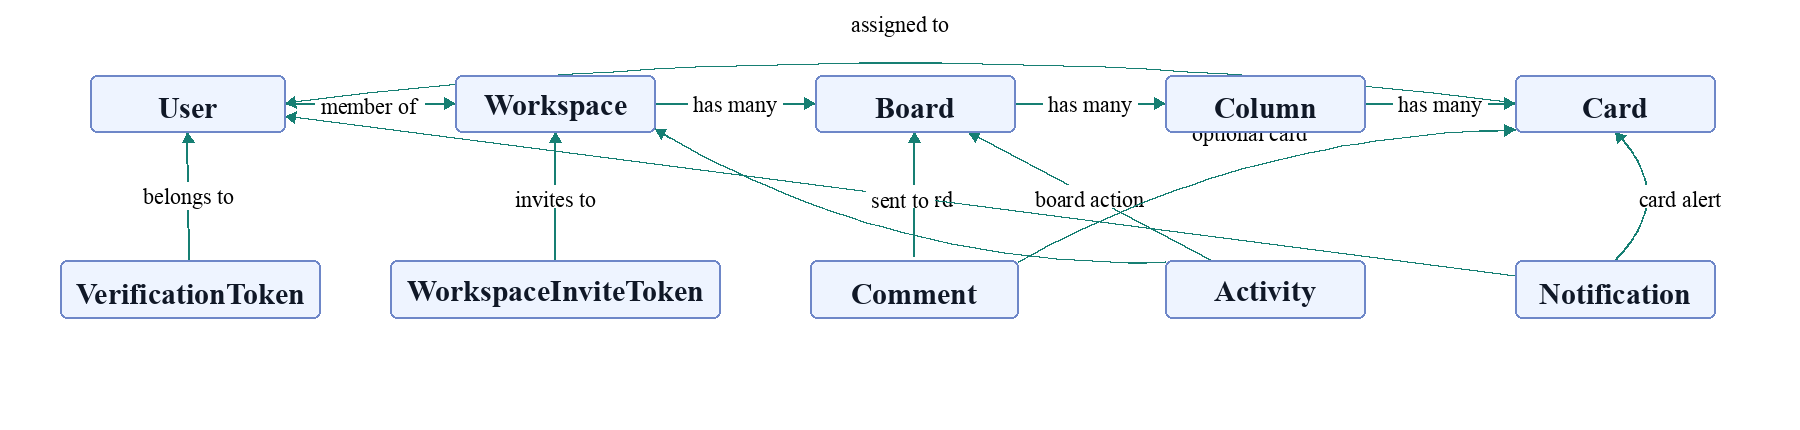
\includegraphics[keepaspectratio,alt={TeamOps ER diagram showing users, workspaces, boards, columns, cards, comments, activity, notifications, and tokens}]{screenshots/teamops-er-diagram.png}}
\caption{TeamOps ER diagram showing users, workspaces, boards, columns,
cards, comments, activity, notifications, and tokens}
\end{figure}

\subsubsection{Why MongoDB Fits This
Project}\label{why-mongodb-fits-this-project}

MongoDB is suitable because the app has nested, document-friendly
entities such as workspace members and fast-changing collaborative board
data. Mongoose schemas still provide structure, indexes, validation, and
model-level consistency. The project uses references for relationships
that need independent queries, such as cards, columns, comments, users,
boards, and activities.

\subsection{Backend Design}\label{backend-design}

\subsubsection{Server Setup}\label{server-setup}

The backend entry point is \texttt{teamops-backend/server.js}. It:

\begin{itemize}
\tightlist
\item
  Loads environment variables.
\item
  Creates an Express app and HTTP server.
\item
  Attaches Socket.io to the same HTTP server.
\item
  Configures CORS with local development support.
\item
  Adds JSON request parsing.
\item
  Registers REST route modules.
\item
  Exposes a \texttt{/api/health} endpoint.
\item
  Connects to MongoDB.
\item
  Seeds sample data if the database is empty and the environment is not
  production.
\item
  Starts the server.
\end{itemize}

\subsubsection{REST API Modules}\label{rest-api-modules}

{\def\LTcaptype{} % do not increment counter
\begin{longtable}[]{@{}
  >{\raggedright\arraybackslash}p{(\linewidth - 2\tabcolsep) * \real{0.5000}}
  >{\raggedright\arraybackslash}p{(\linewidth - 2\tabcolsep) * \real{0.5000}}@{}}
\toprule\noalign{}
\begin{minipage}[b]{\linewidth}\raggedright
Route Prefix
\end{minipage} & \begin{minipage}[b]{\linewidth}\raggedright
Responsibility
\end{minipage} \\
\midrule\noalign{}
\endhead
\bottomrule\noalign{}
\endlastfoot
\texttt{/api/auth} & Register, login, verify, resend verification,
Google login, forgot/reset password, current user \\
\texttt{/api/workspaces} & Workspace CRUD, members, roles, invite code
joining, email invite joining, workspace boards \\
\texttt{/api/boards} & Board data, analytics, comments, columns, cards,
movement \\
\texttt{/api/activities} & Activity timeline and audit views \\
\texttt{/api/notifications} & Notification inbox, unread count, mark
read, mark all read, important flag \\
\texttt{/api/user} & Profile, password change, assigned cards \\
\end{longtable}
}

\subsubsection{Authentication Flow}\label{authentication-flow}

For email registration:

\begin{enumerate}
\def\labelenumi{\arabic{enumi}.}
\tightlist
\item
  User submits name, email, and password.
\item
  Backend trims and normalizes data.
\item
  Password is hashed with bcrypt.
\item
  User is created as unverified.
\item
  Six-digit OTP is generated and stored in \texttt{VerificationToken}.
\item
  Verification email is sent.
\item
  User enters OTP.
\item
  Backend verifies token and expiry.
\item
  User becomes verified.
\item
  JWT is issued in an HTTP-only cookie for a seven-day session.
\end{enumerate}

For login:

\begin{enumerate}
\def\labelenumi{\arabic{enumi}.}
\tightlist
\item
  User submits email and password.
\item
  Backend finds the normalized email.
\item
  Backend rejects unknown, unverified, or Google-only accounts where
  appropriate.
\item
  bcrypt compares the submitted password with the stored hash.
\item
  A signed JWT session cookie is set.
\end{enumerate}

For Google login:

\begin{enumerate}
\def\labelenumi{\arabic{enumi}.}
\tightlist
\item
  Frontend receives a Google credential.
\item
  Backend verifies the ID token using Google Auth Library.
\item
  Backend extracts Google id, email, name, and avatar.
\item
  Existing user is updated or a new Google user is created.
\item
  The same workspace setup flow is used as email signup: if no workspace
  exists, the user is asked to create or join one.
\item
  A signed JWT session cookie is set.
\end{enumerate}

\subsubsection{Authorization and RBAC}\label{authorization-and-rbac}

TeamOps uses workspace roles:

{\def\LTcaptype{} % do not increment counter
\begin{longtable}[]{@{}
  >{\raggedright\arraybackslash}p{(\linewidth - 4\tabcolsep) * \real{0.3000}}
  >{\raggedleft\arraybackslash}p{(\linewidth - 4\tabcolsep) * \real{0.4000}}
  >{\raggedright\arraybackslash}p{(\linewidth - 4\tabcolsep) * \real{0.3000}}@{}}
\toprule\noalign{}
\begin{minipage}[b]{\linewidth}\raggedright
Role
\end{minipage} & \begin{minipage}[b]{\linewidth}\raggedleft
Level
\end{minipage} & \begin{minipage}[b]{\linewidth}\raggedright
Typical Permissions
\end{minipage} \\
\midrule\noalign{}
\endhead
\bottomrule\noalign{}
\endlastfoot
owner & 3 & Full workspace control, delete workspace, manage all
members \\
admin & 2 & Manage boards, columns, members, settings, invites \\
member & 1 & Create/edit/move cards, comment, collaborate \\
viewer & 0 & Read board data and comments, limited interaction \\
\end{longtable}
}

The backend uses both route middleware and controller-level checks. The
\texttt{requireRole} middleware resolves the workspace from route params
or related board/column/card ids, then validates that the current user
has one of the required roles. Controllers also use helper functions
such as \texttt{checkWorkspaceAccess} and \texttt{resolveBoardAccess} to
enforce role hierarchy before sensitive operations.

\subsubsection{Real-Time Design}\label{real-time-design}

Socket.io is initialized in \texttt{server.js} and handled in
\texttt{socket/index.js}. During connection, the server parses the
session cookie from the socket handshake headers and verifies the JWT.
If valid, it joins a private
\texttt{user:\textless{}userId\textgreater{}} room.

The frontend joins board and workspace rooms:

\begin{itemize}
\tightlist
\item
  \texttt{board:join} or \texttt{join:board} to subscribe to board
  updates.
\item
  \texttt{workspace:join} or \texttt{join:workspace} to subscribe to
  presence count.
\item
  \texttt{join:user} for private notification delivery.
\end{itemize}

Important emitted events include:

{\def\LTcaptype{} % do not increment counter
\begin{longtable}[]{@{}ll@{}}
\toprule\noalign{}
Event & Use \\
\midrule\noalign{}
\endhead
\bottomrule\noalign{}
\endlastfoot
\texttt{card:created} & A new card was added \\
\texttt{card:updated} & Card details changed \\
\texttt{card:deleted} & Card removed \\
\texttt{card:moved} & Card moved to another column/position \\
\texttt{column:created} & Board column added \\
\texttt{column:deleted} & Board column removed \\
\texttt{card:commented} & Card comment created \\
\texttt{comment:deleted} & Card comment deleted \\
\texttt{board:commented} & Board comment created \\
\texttt{board:comment:deleted} & Board comment deleted \\
\texttt{activity:new} & Timeline event created \\
\texttt{notification:new} & User notification created \\
\texttt{workspace:presence} & Current active connection count for
workspace \\
\end{longtable}
}

\subsection{Frontend Design}\label{frontend-design}

The frontend is a standalone app inside
\texttt{teamops-frontend/index.html} and
\texttt{teamops-frontend/styles.css}. It does not use React components.
The app uses DOM functions, \texttt{fetch}, local state variables,
browser cookies for authentication, limited \texttt{localStorage} for
non-sensitive UI/workspace context, custom modals, custom select
controls, and Socket.io client events.

Main frontend responsibilities:

\begin{itemize}
\tightlist
\item
  Switching views such as landing, auth, workspace setup, join
  workspace, and dashboard.
\item
  Managing authentication forms and verification/reset flows.
\item
  Keeping only non-sensitive UI context in \texttt{localStorage}, such
  as selected workspace/board ids and saved views.
\item
  Calling REST endpoints through a shared \texttt{apiRequest} helper
  with
  \texttt{credentials:\ \textquotesingle{}include\textquotesingle{}} and
  CSRF headers for unsafe requests.
\item
  Connecting to Socket.io and subscribing to board/user/workspace rooms.
\item
  Rendering boards, columns, cards, filters, comments, activity,
  notifications, members, analytics, profile, and saved views.
\item
  Enforcing role-based UI restrictions so viewers cannot
  create/edit/delete cards or columns.
\item
  Providing drag-and-drop behavior for card movement.
\item
  Showing toast feedback and confirmation dialogs.
\item
  Supporting dashboard pages for projects, roadmap, integrations,
  channels, help, saved views, profile, workspace settings, and audit
  logs.
\end{itemize}

\subsection{Application Screenshots}\label{application-screenshots}

The following screenshots document the main user-facing output of
TeamOps. They show the public entry screen, authentication flow,
workspace onboarding, dashboard shell, empty board state, analytics,
members page, workspace settings, and card creation workflow.

\begin{figure}
\centering
\pandocbounded{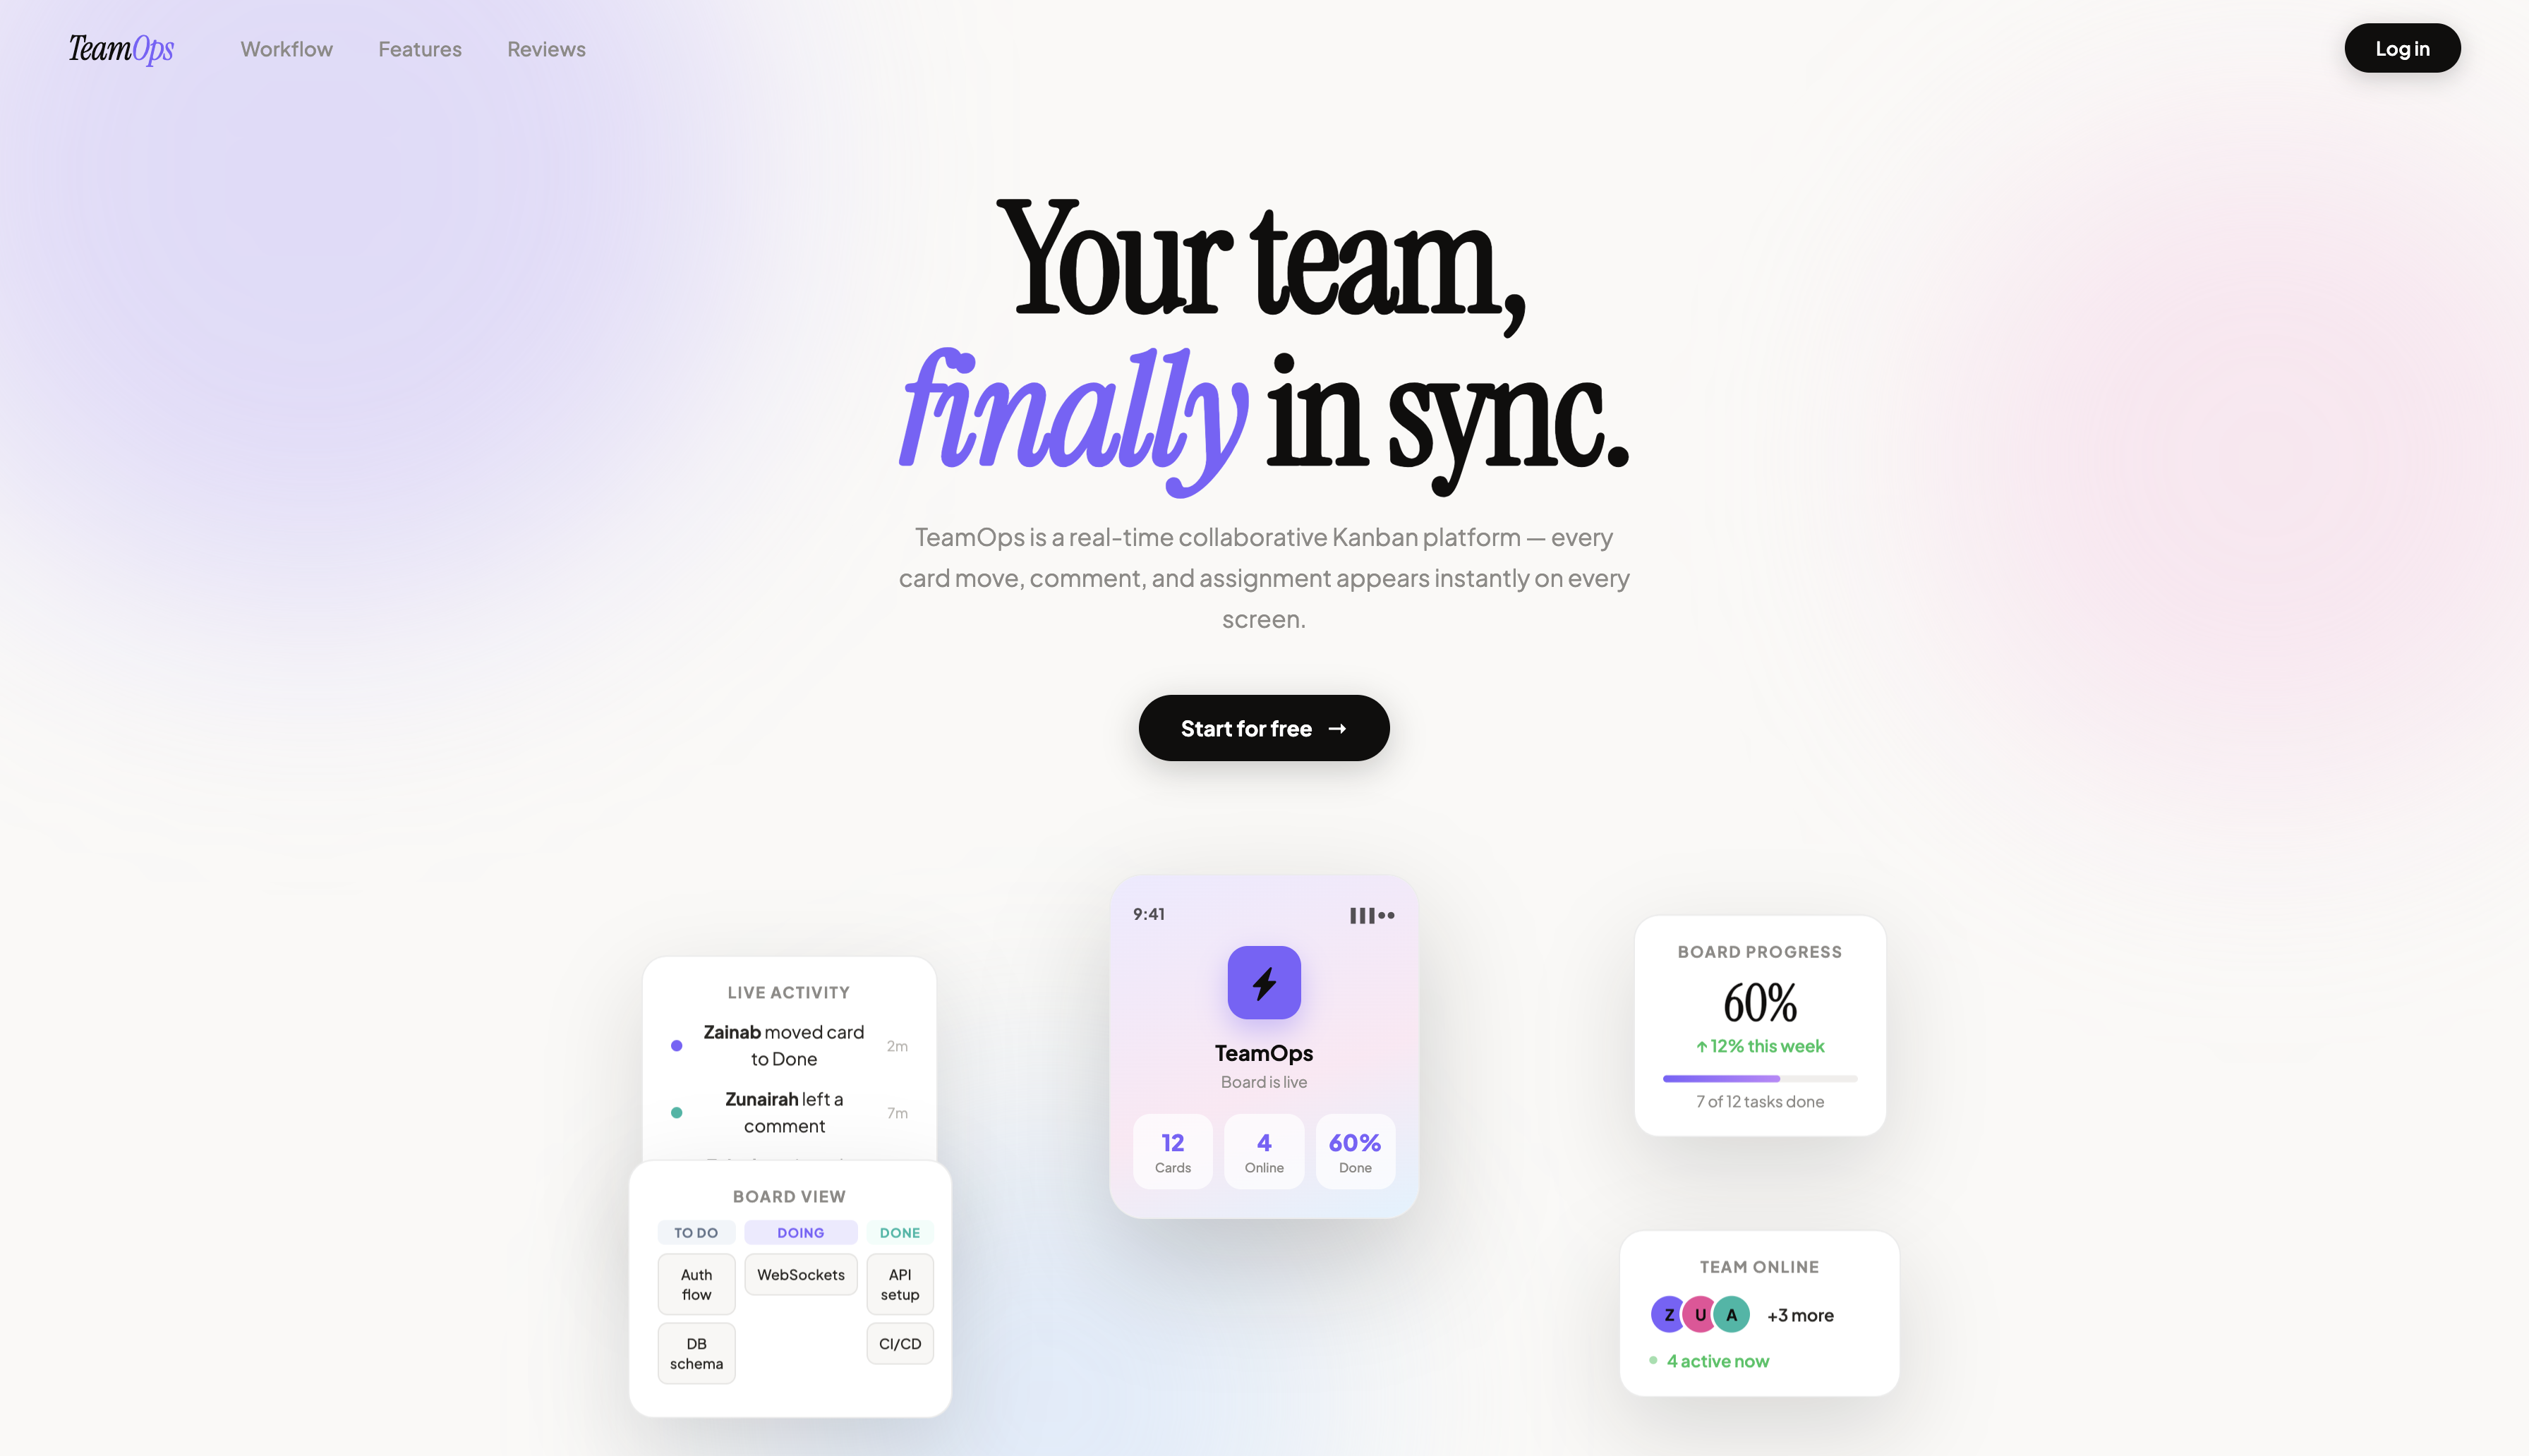
\includegraphics[keepaspectratio,alt={Landing page and product overview}]{screenshots/report-landing.png}}
\caption{Landing page and product overview}
\end{figure}

\begin{figure}
\centering
\pandocbounded{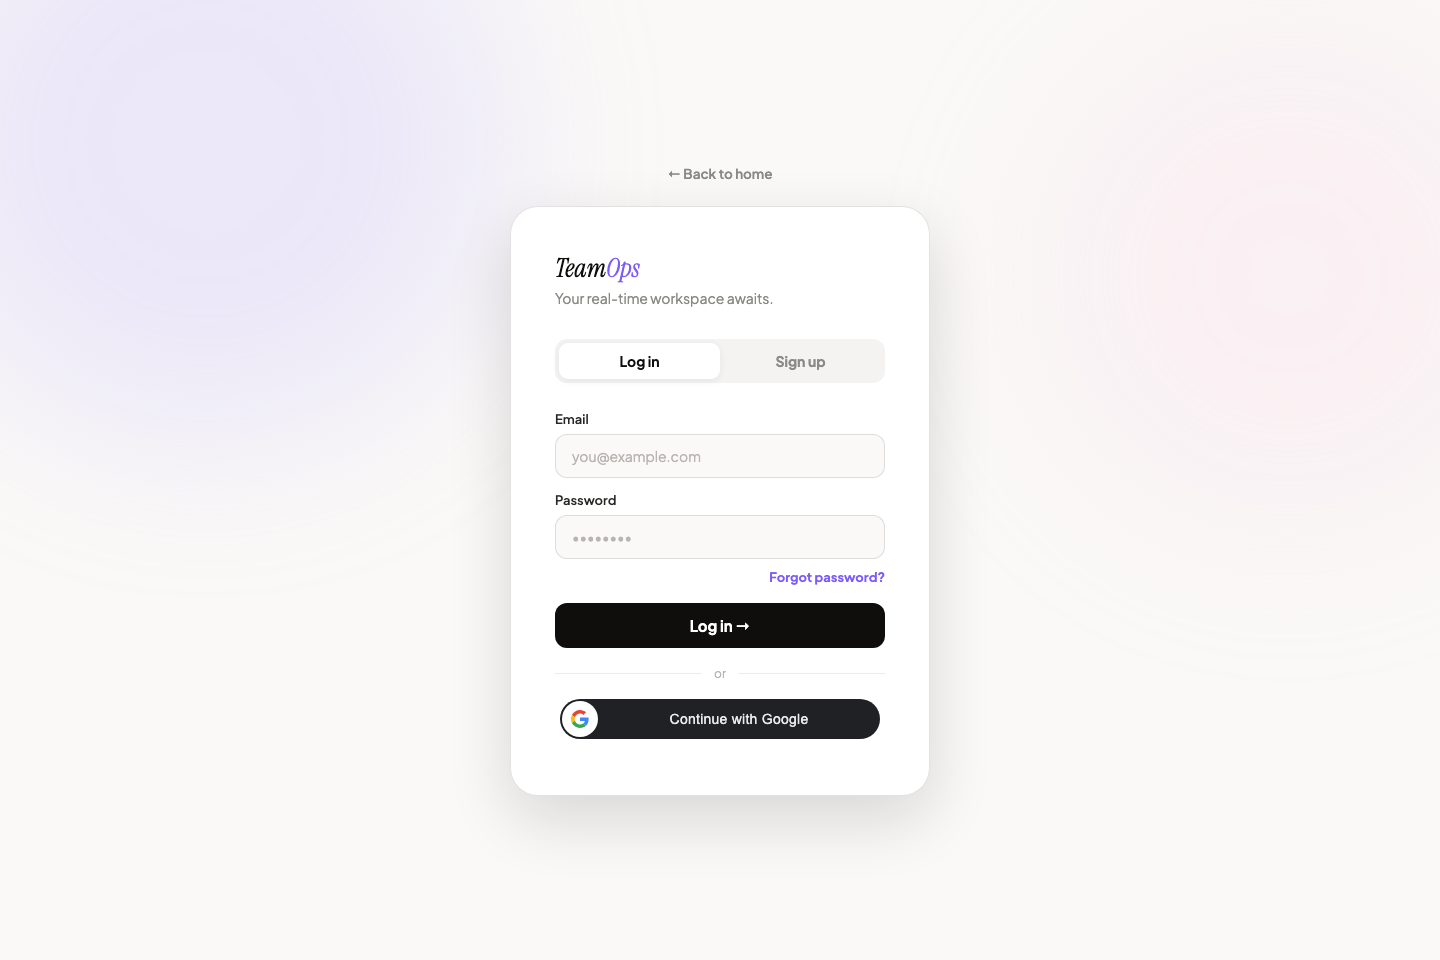
\includegraphics[keepaspectratio,alt={Initial landing screen}]{screenshots/landing-page.png}}
\caption{Initial landing screen}
\end{figure}

\begin{figure}
\centering
\pandocbounded{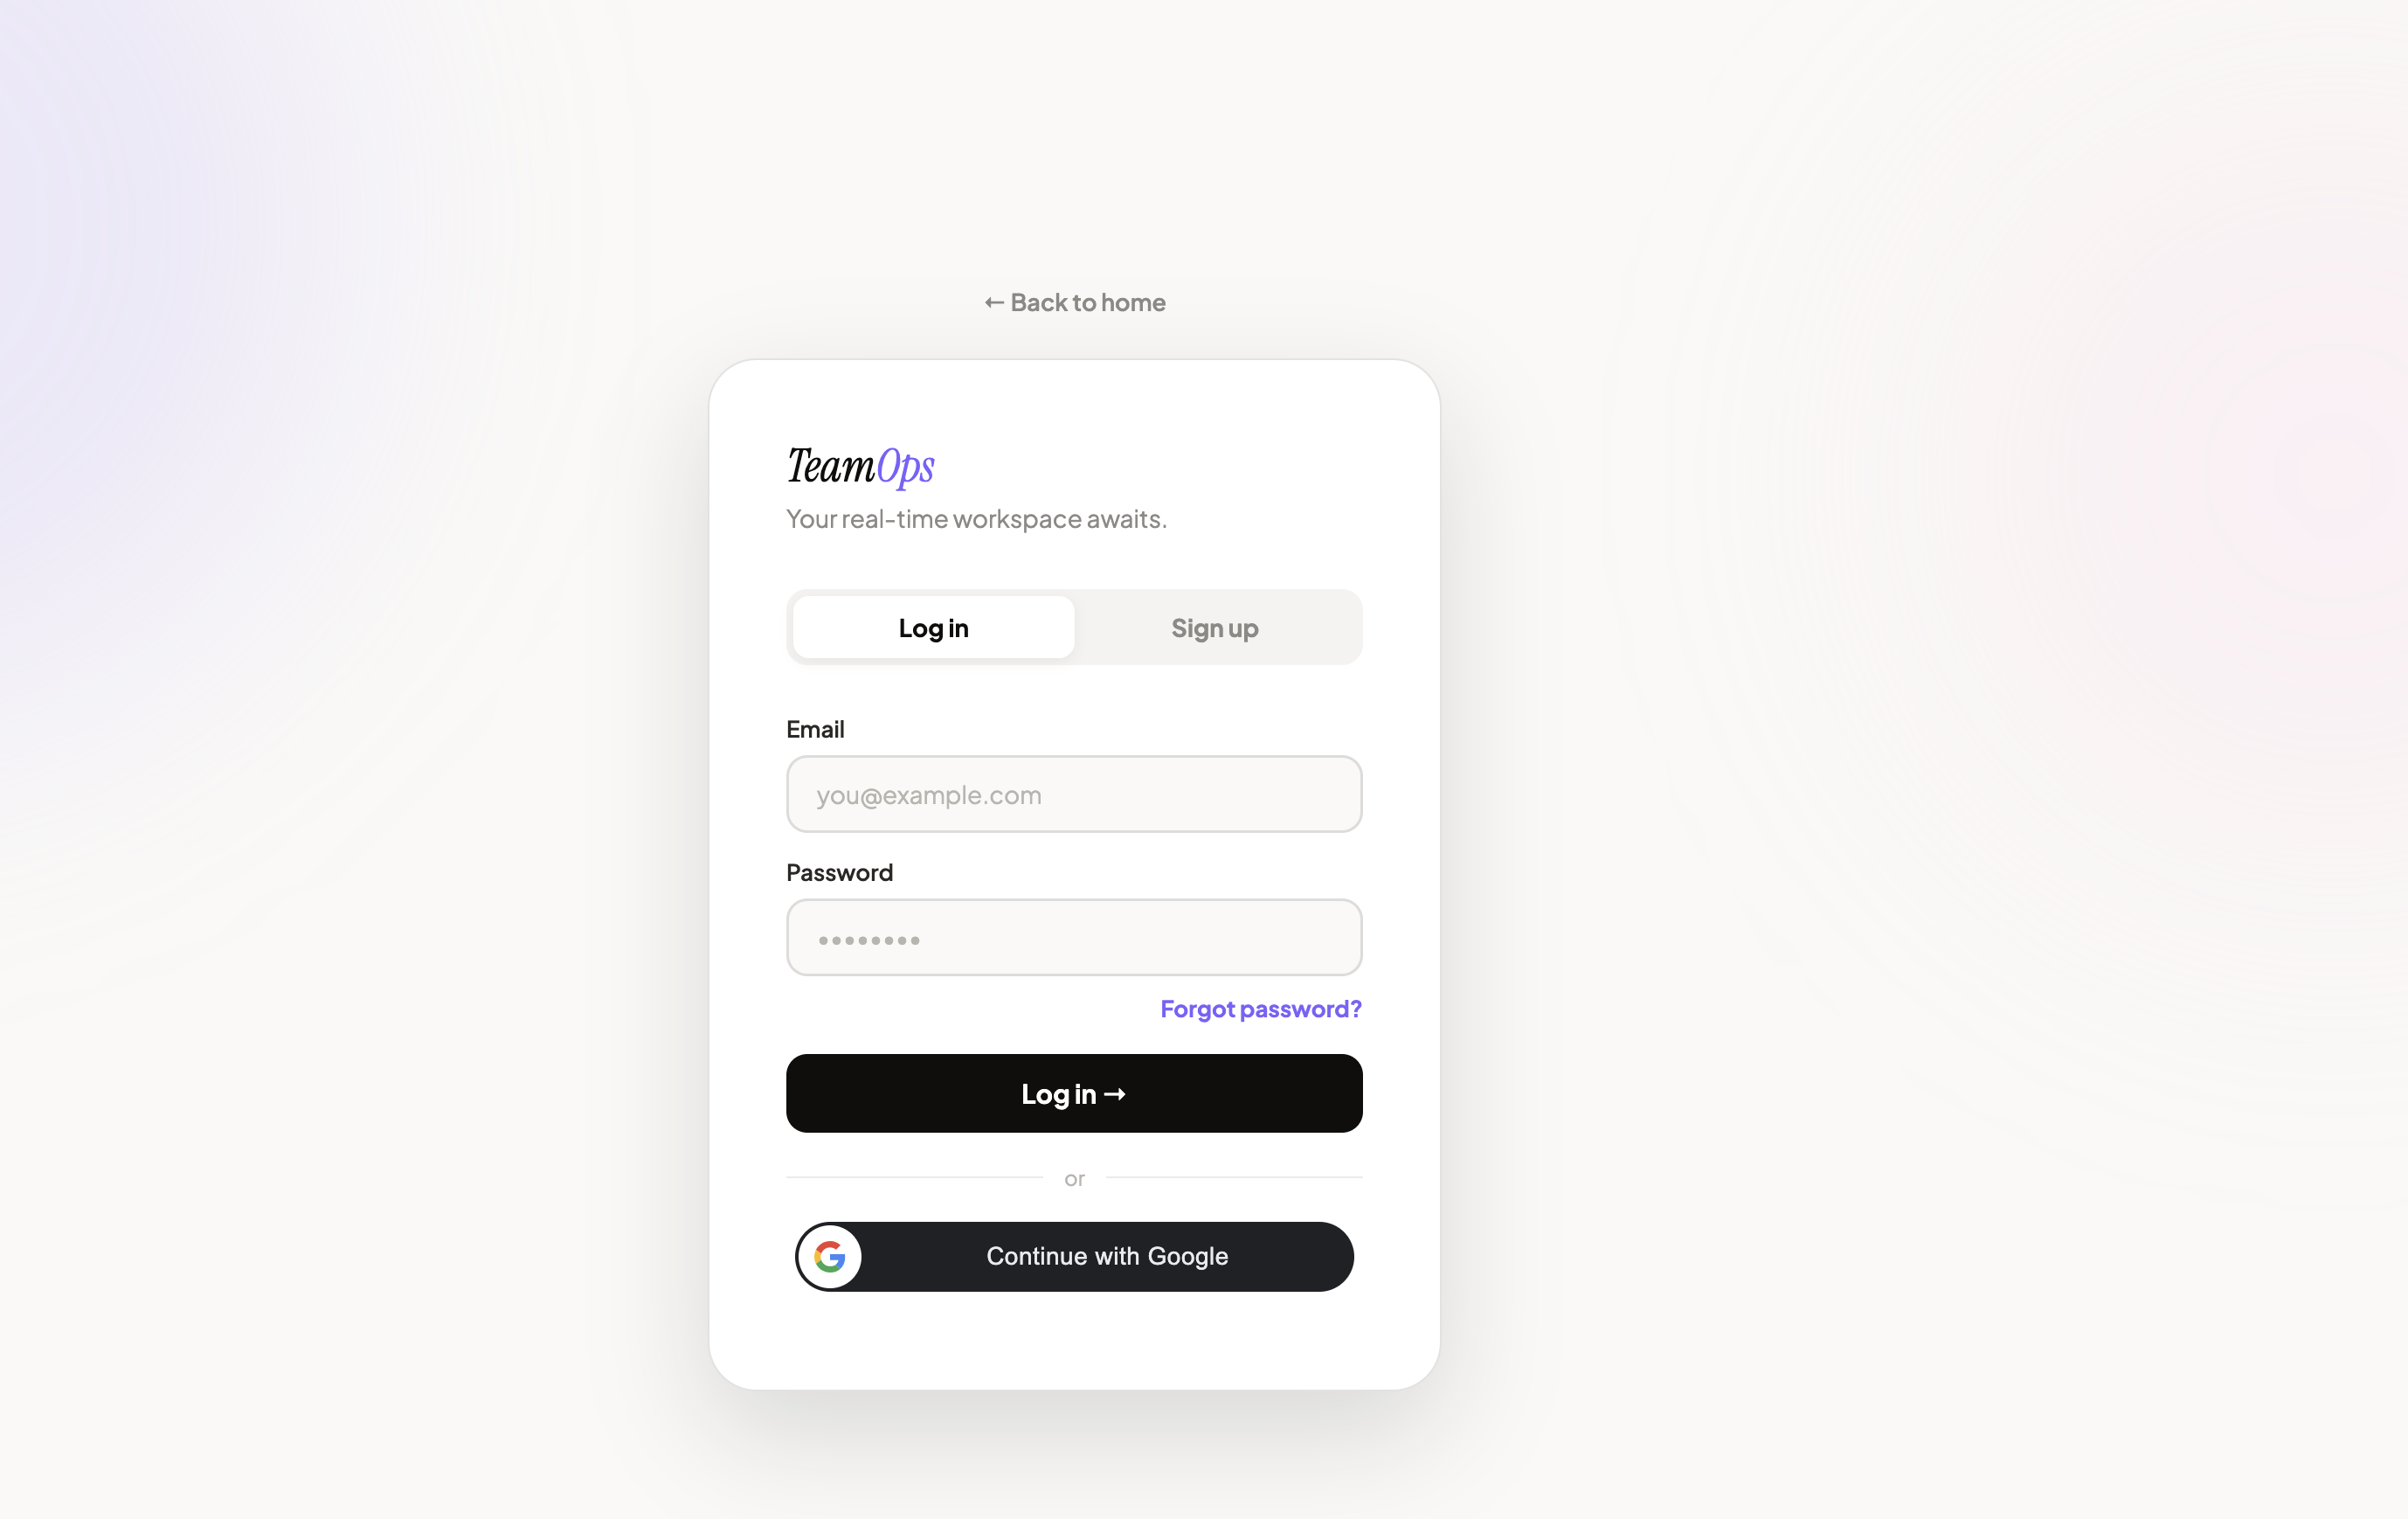
\includegraphics[keepaspectratio,alt={Login and Google authentication}]{screenshots/report-login.png}}
\caption{Login and Google authentication}
\end{figure}

\begin{figure}
\centering
\pandocbounded{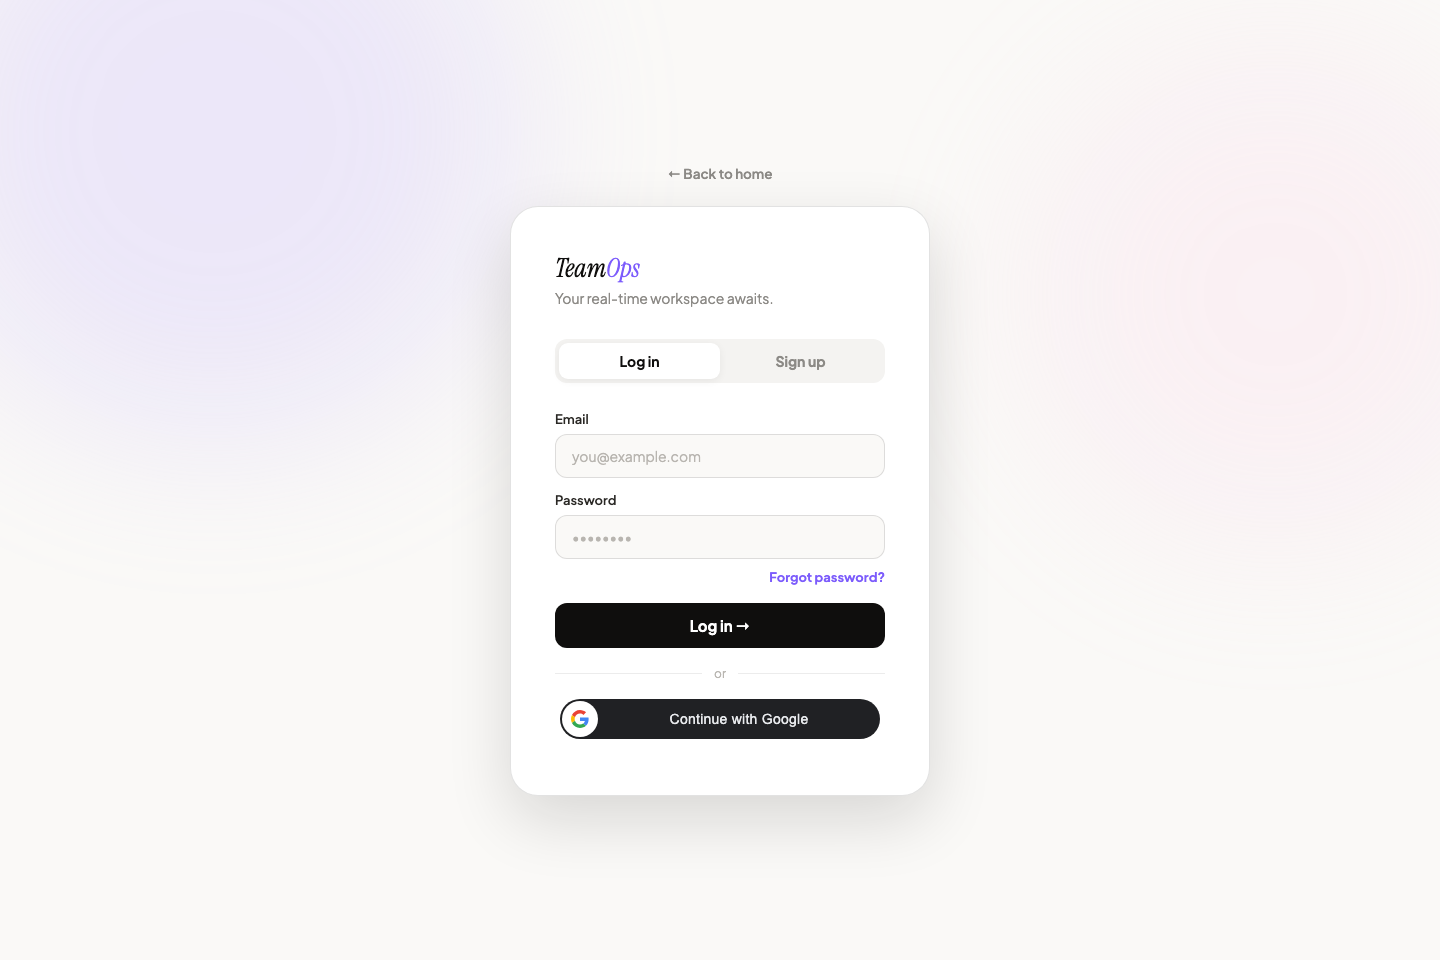
\includegraphics[keepaspectratio,alt={Authentication screen}]{screenshots/auth-screen.png}}
\caption{Authentication screen}
\end{figure}

\begin{figure}
\centering
\pandocbounded{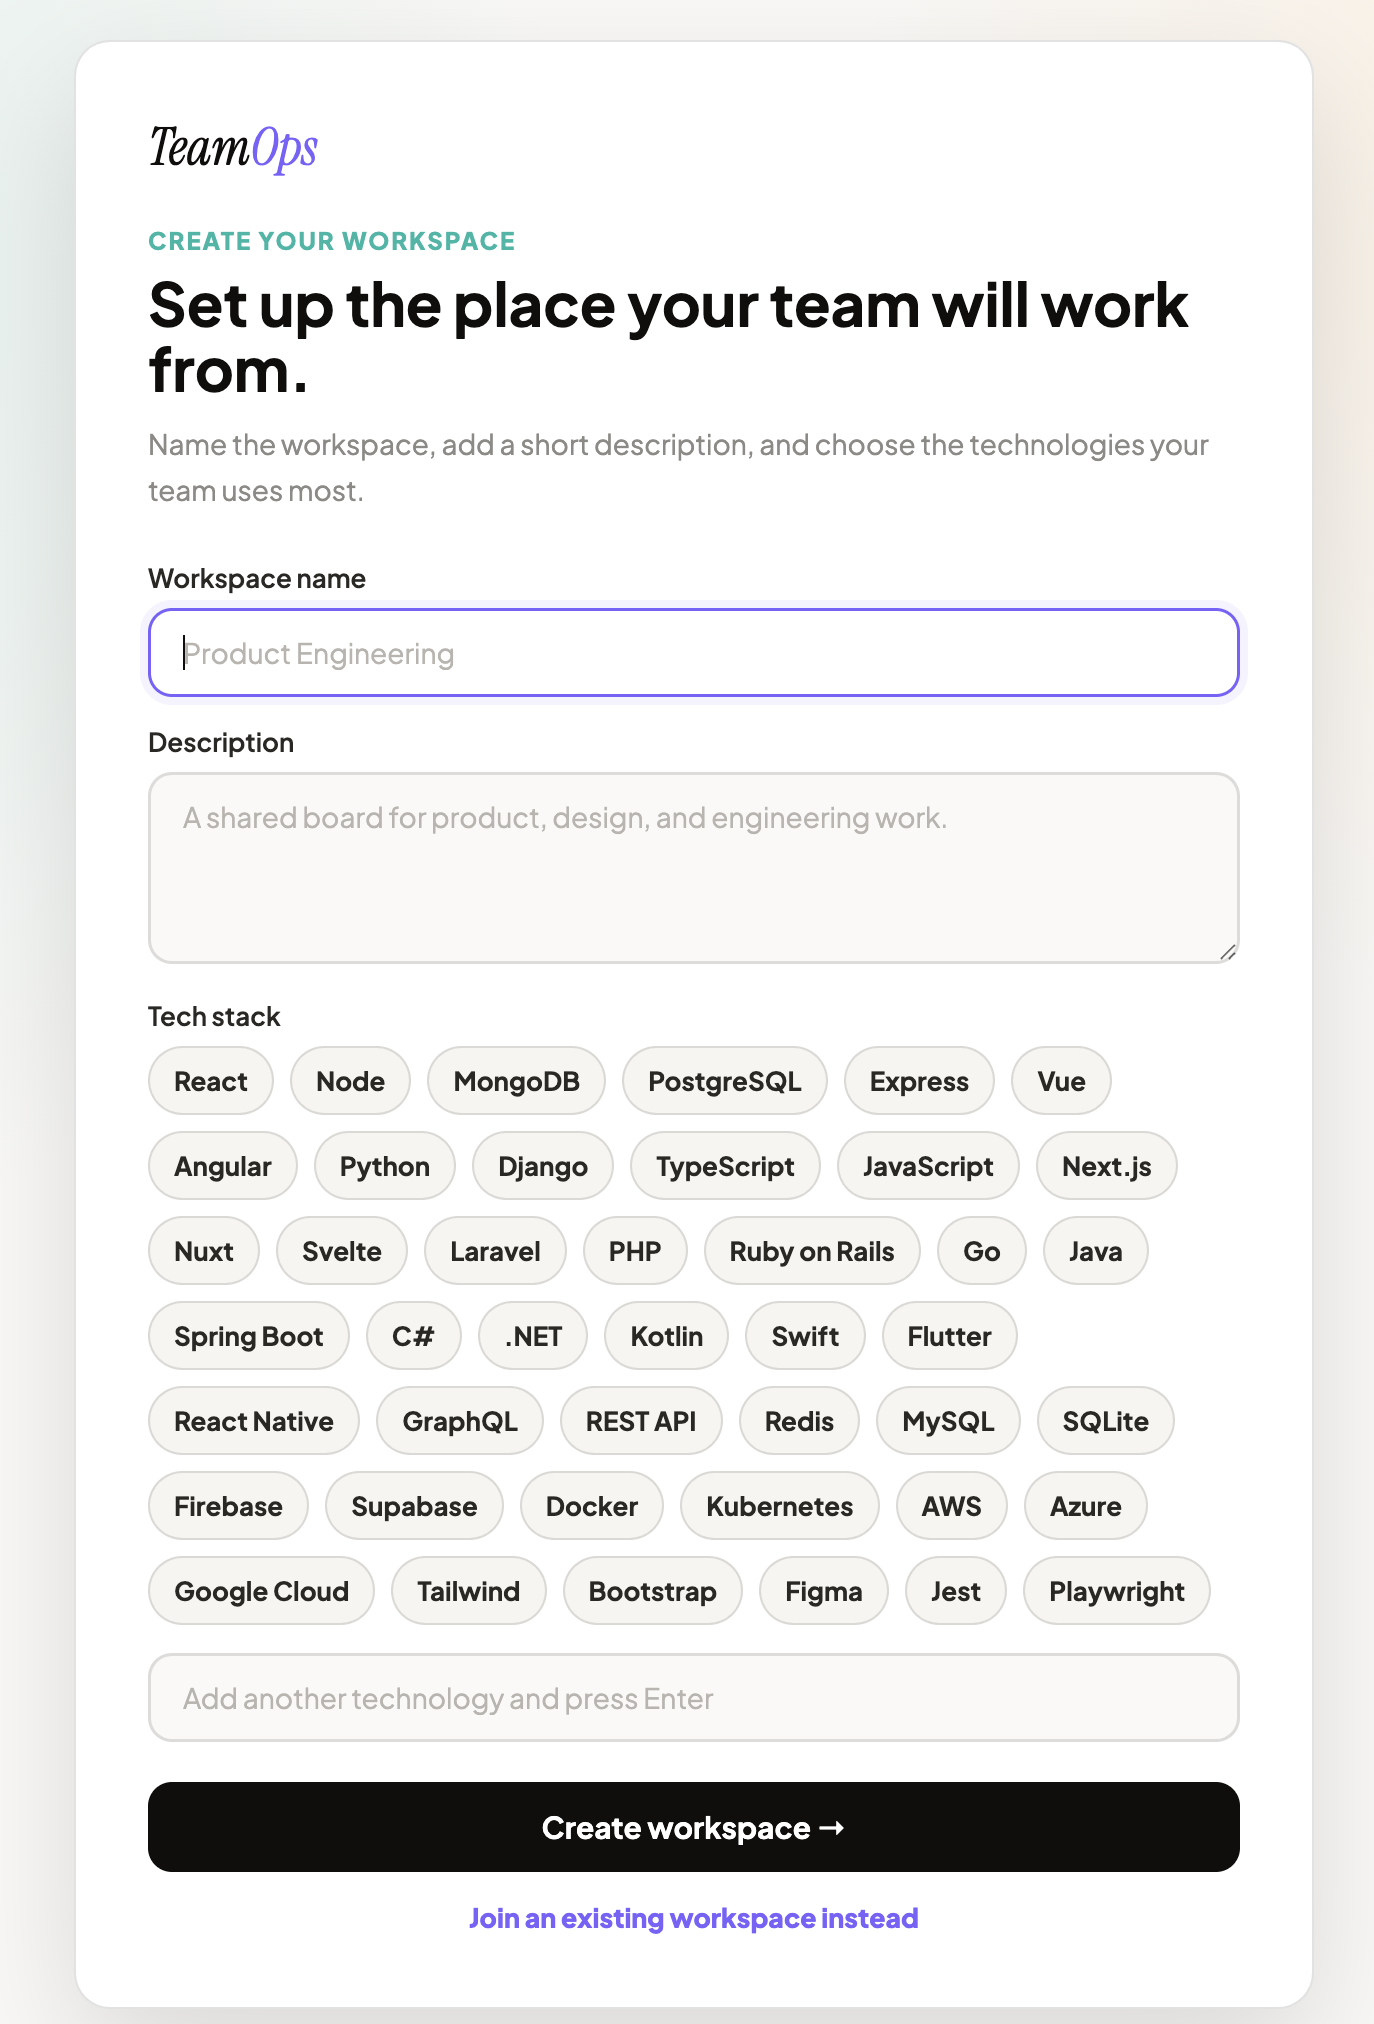
\includegraphics[keepaspectratio,alt={Workspace creation form}]{screenshots/report-workspace-create.png}}
\caption{Workspace creation form}
\end{figure}

\begin{figure}
\centering
\pandocbounded{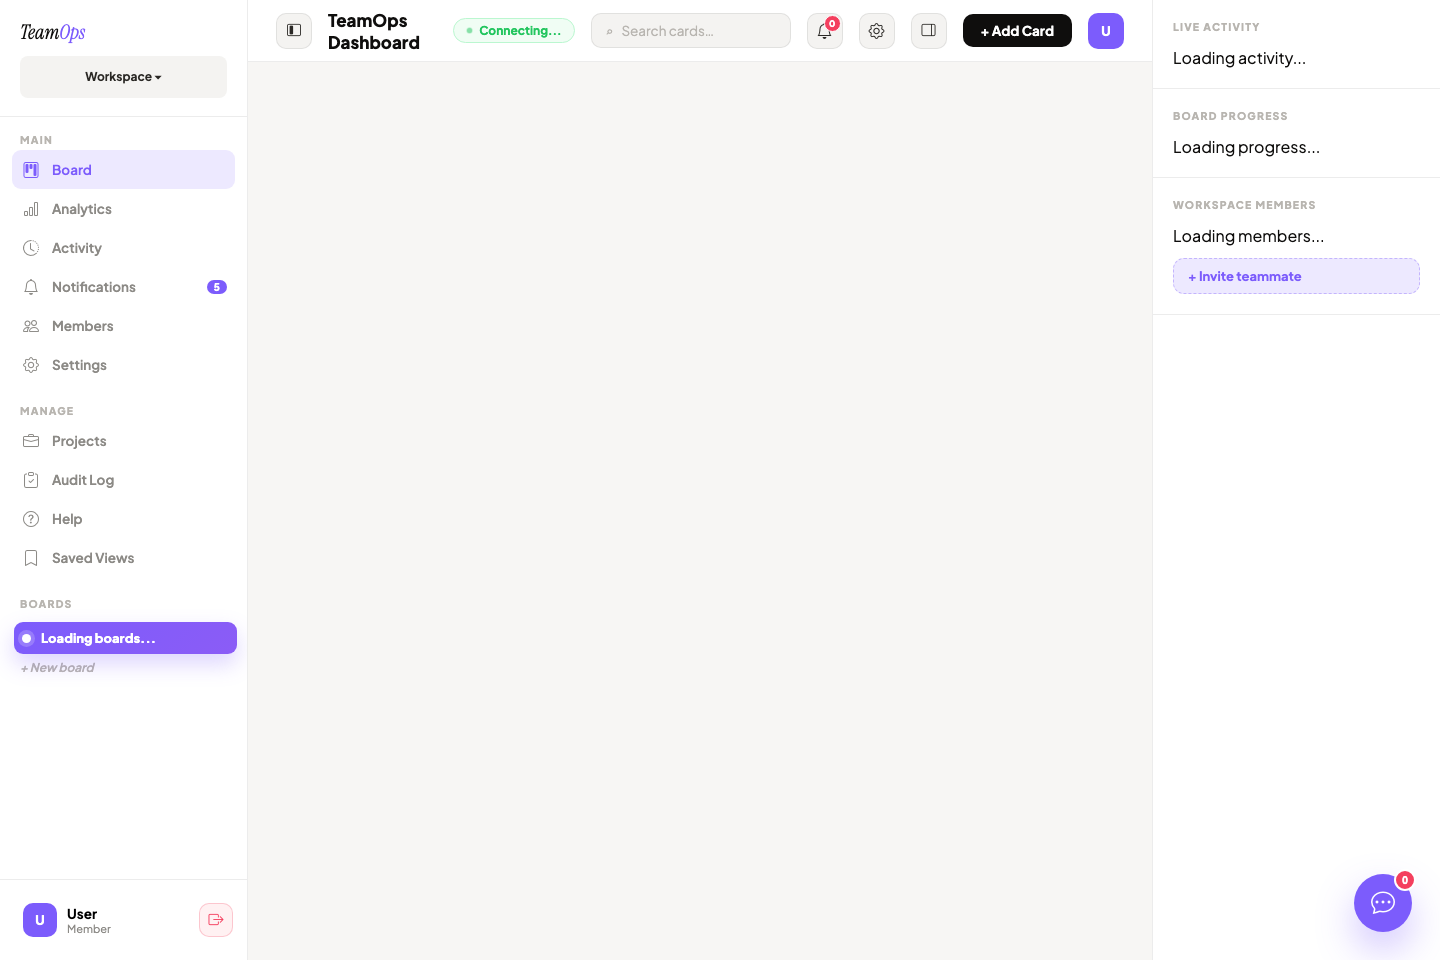
\includegraphics[keepaspectratio,alt={Dashboard shell}]{screenshots/dashboard-shell.png}}
\caption{Dashboard shell}
\end{figure}

\begin{figure}
\centering
\pandocbounded{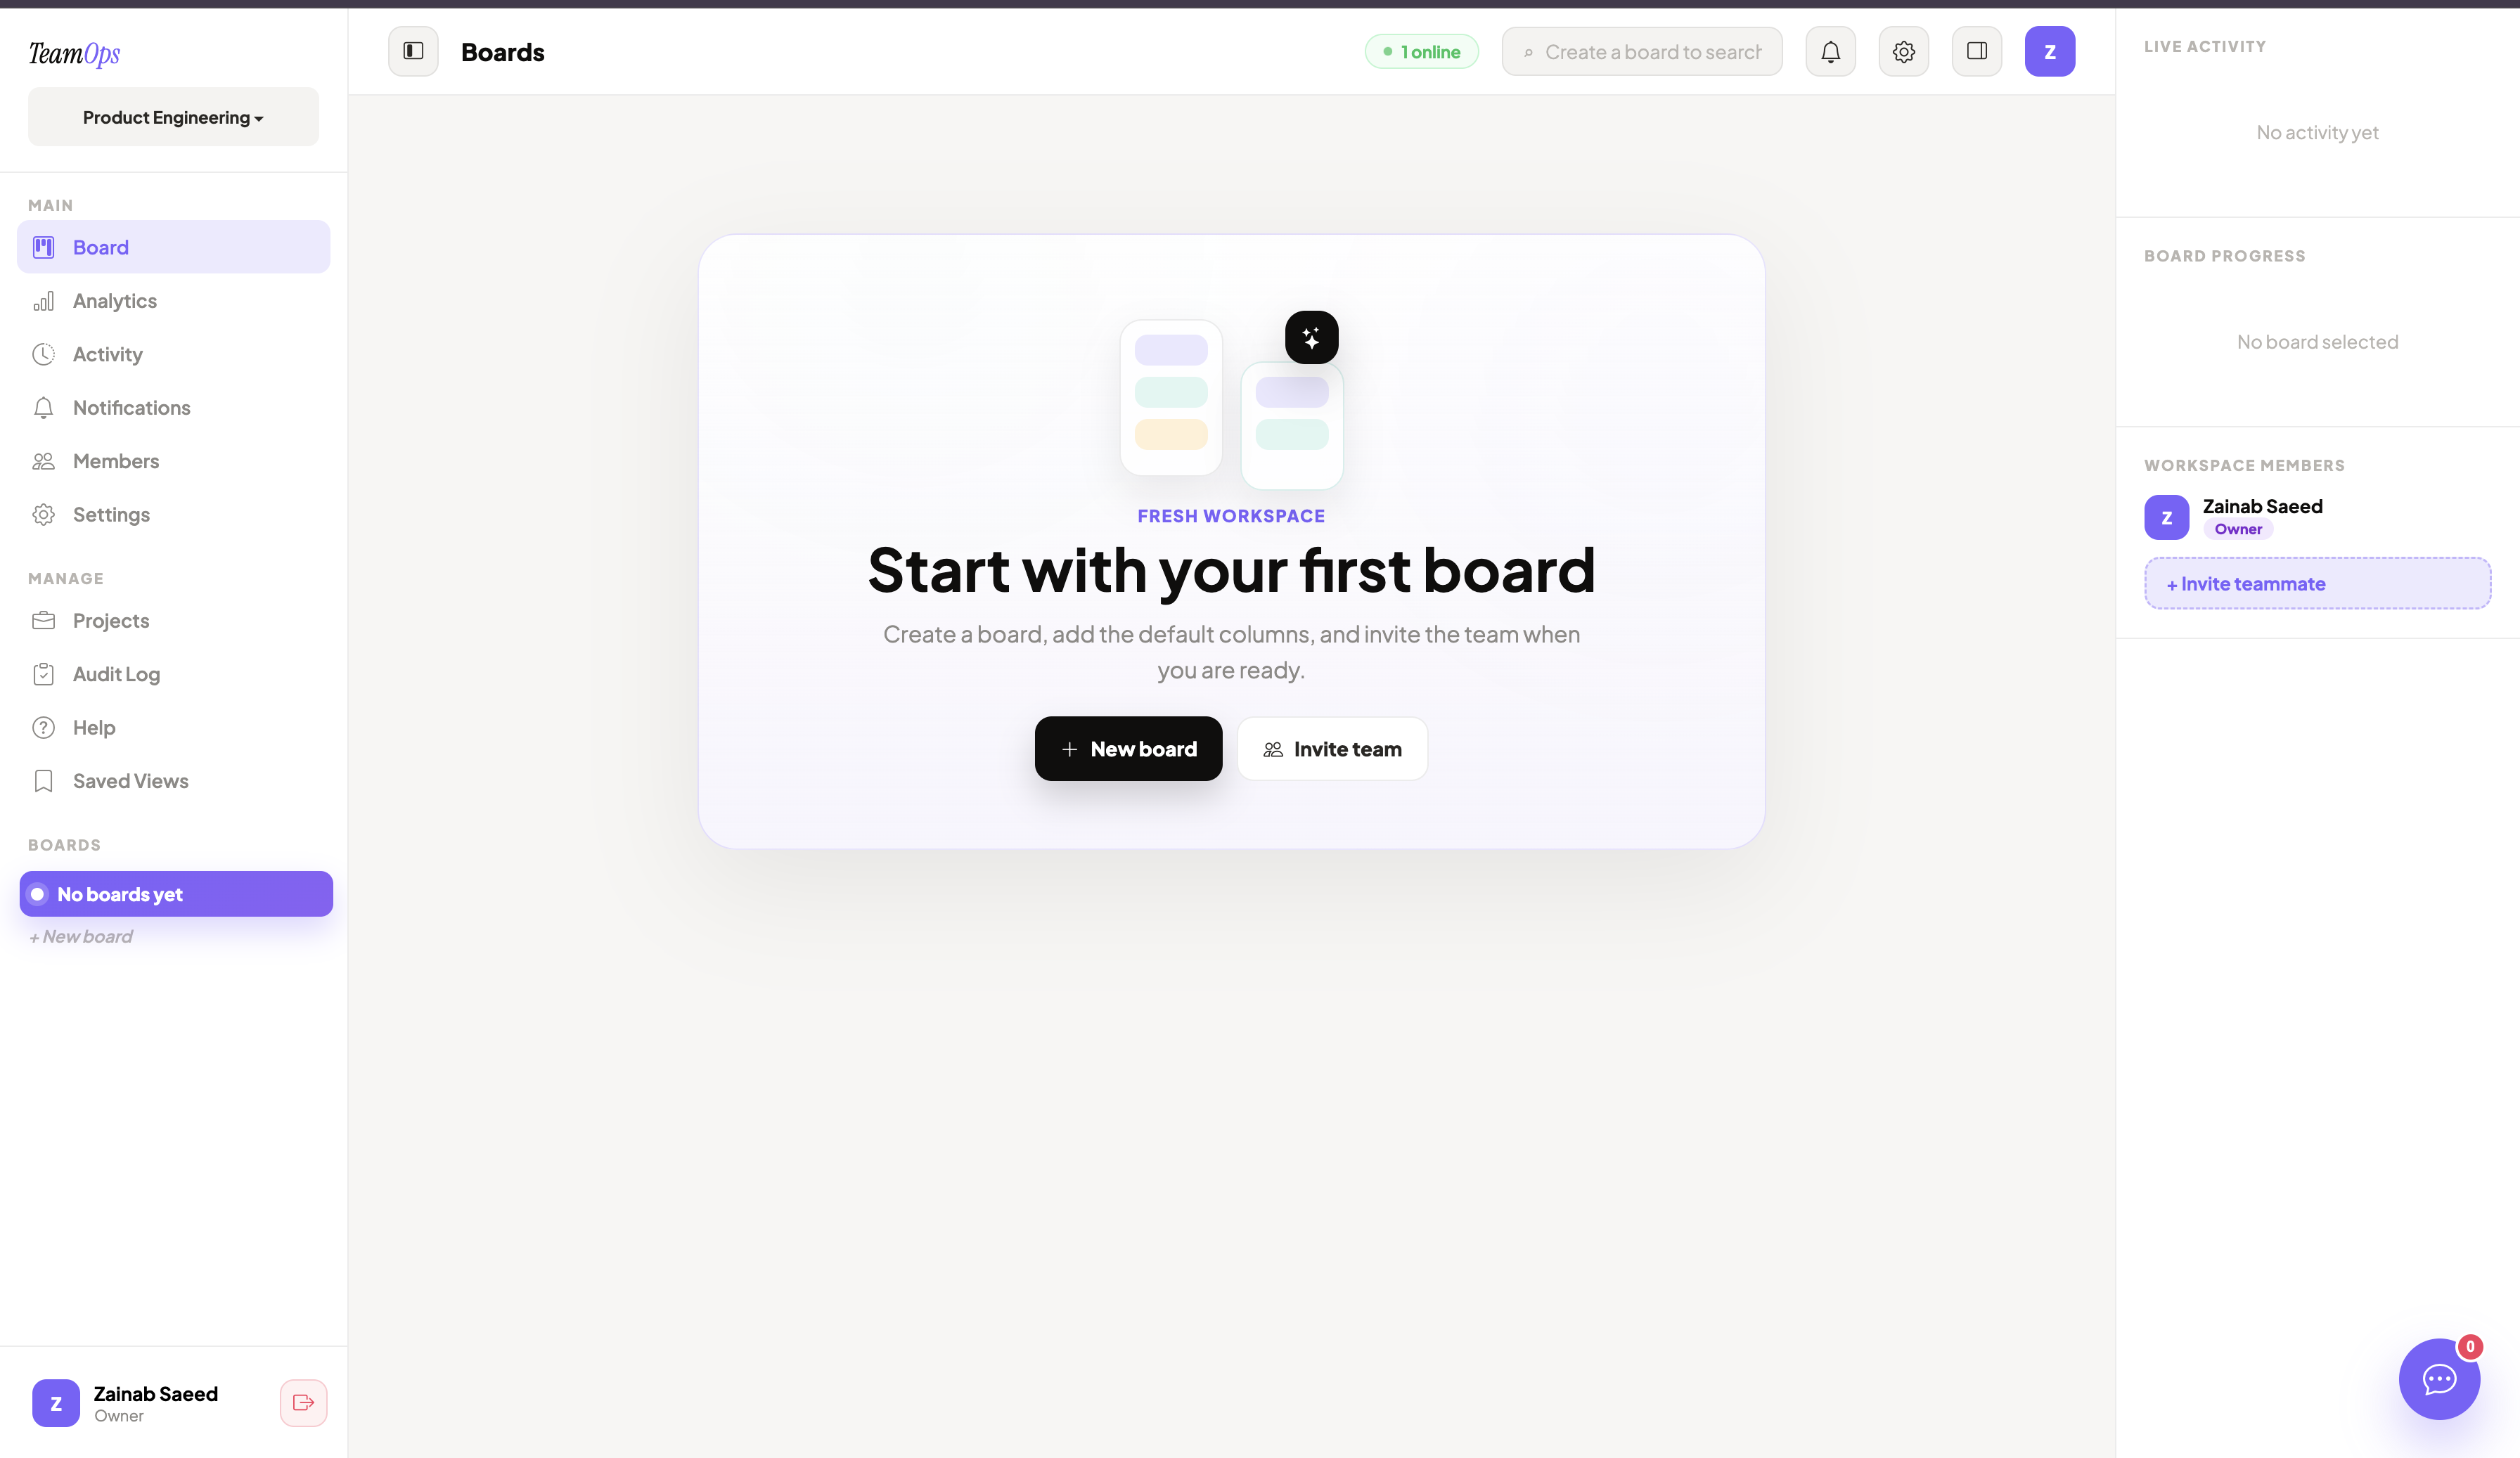
\includegraphics[keepaspectratio,alt={New workspace with no boards yet}]{screenshots/report-empty-board.png}}
\caption{New workspace with no boards yet}
\end{figure}

\begin{figure}
\centering
\pandocbounded{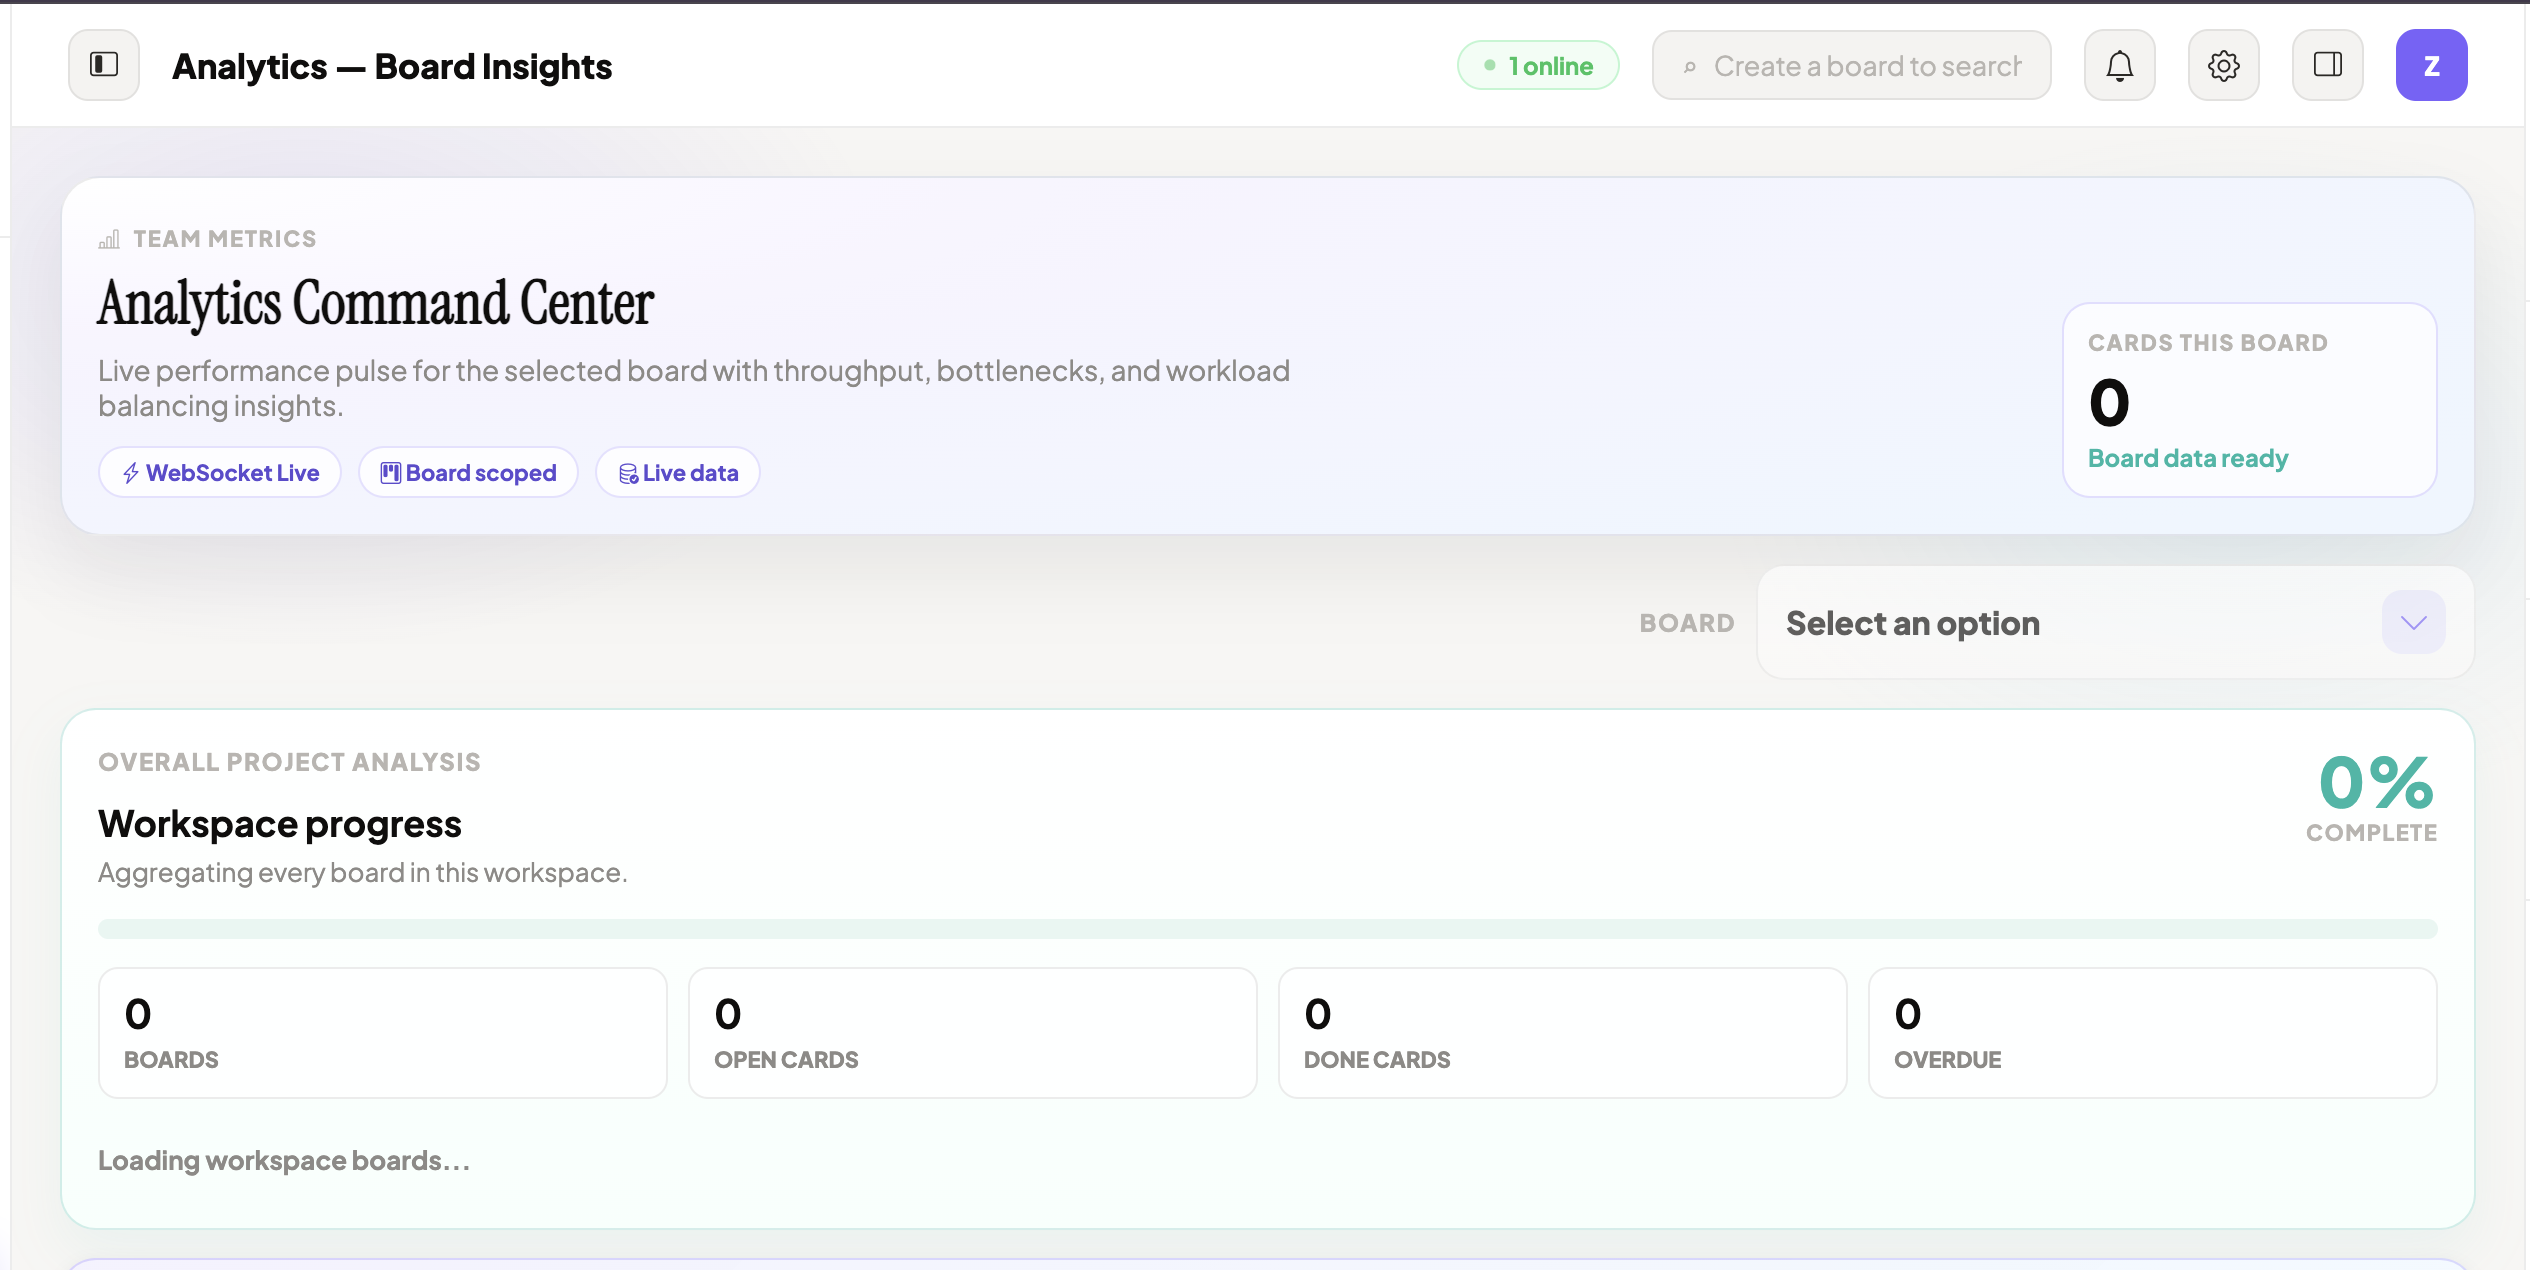
\includegraphics[keepaspectratio,alt={Analytics view for an empty workspace}]{screenshots/report-analytics.png}}
\caption{Analytics view for an empty workspace}
\end{figure}

\begin{figure}
\centering
\pandocbounded{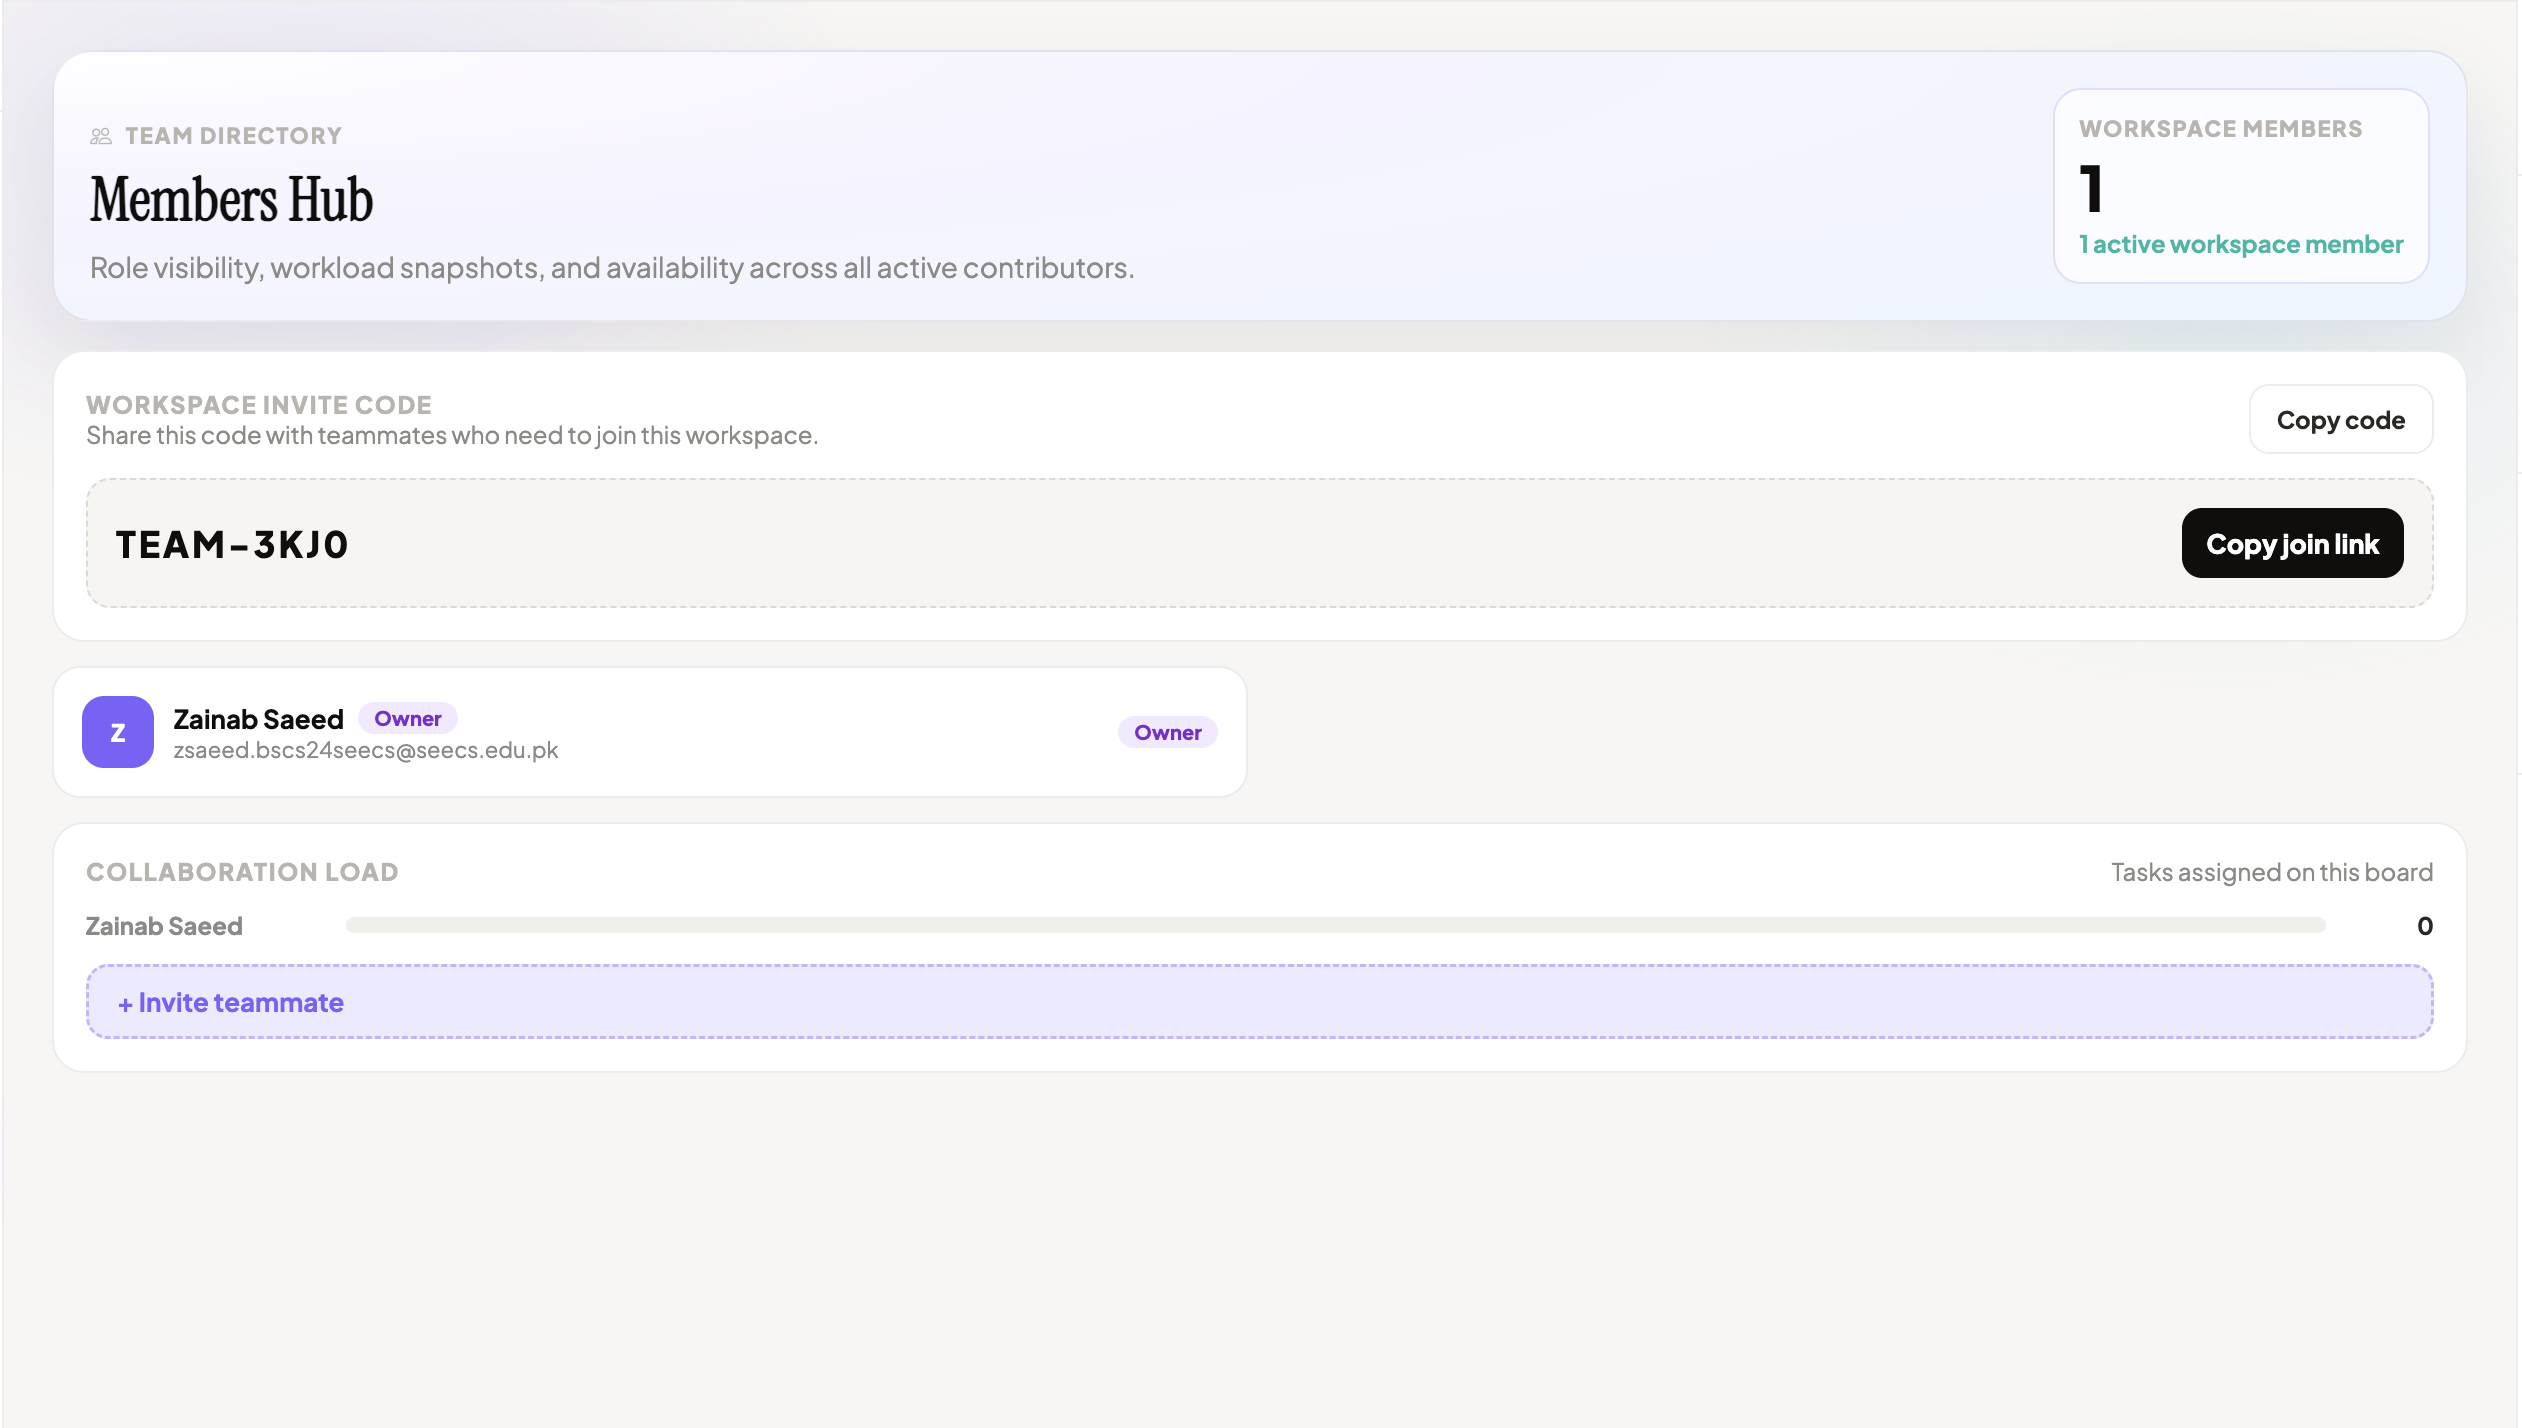
\includegraphics[keepaspectratio,alt={Members and invite code page}]{screenshots/report-members.png}}
\caption{Members and invite code page}
\end{figure}

\begin{figure}
\centering
\pandocbounded{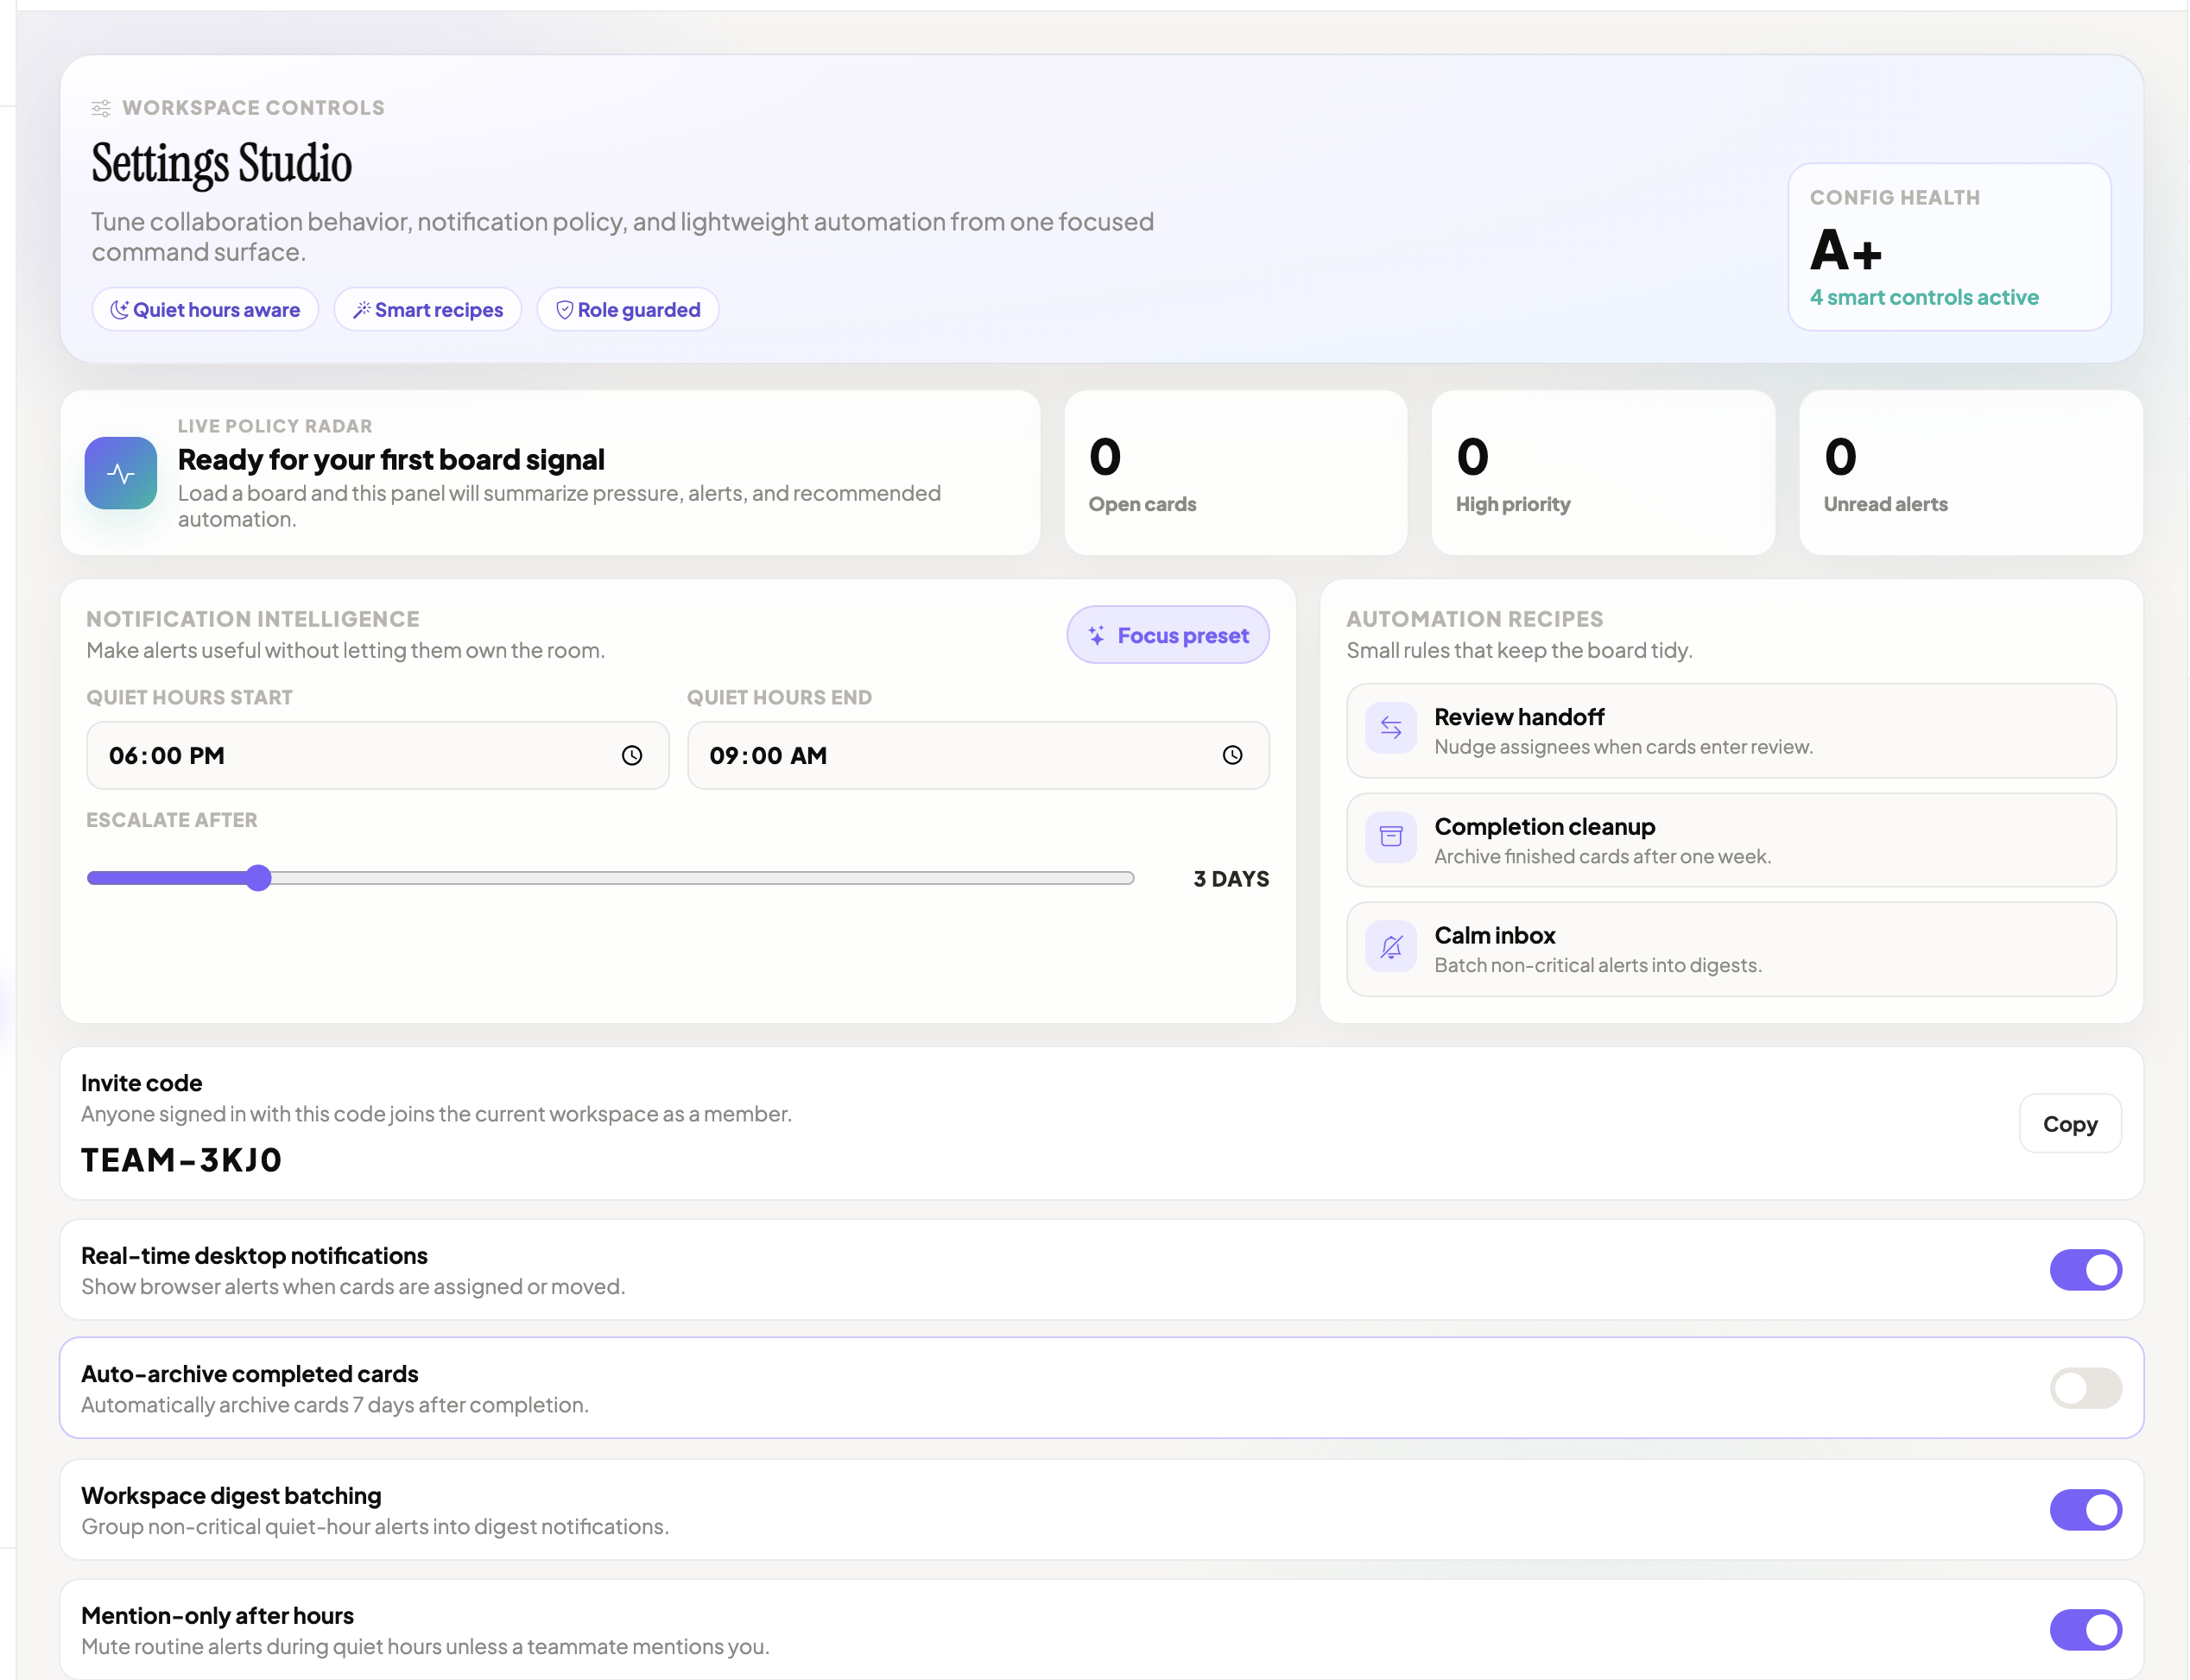
\includegraphics[keepaspectratio,alt={Workspace settings and automation controls}]{screenshots/report-settings.png}}
\caption{Workspace settings and automation controls}
\end{figure}

\begin{figure}
\centering
\pandocbounded{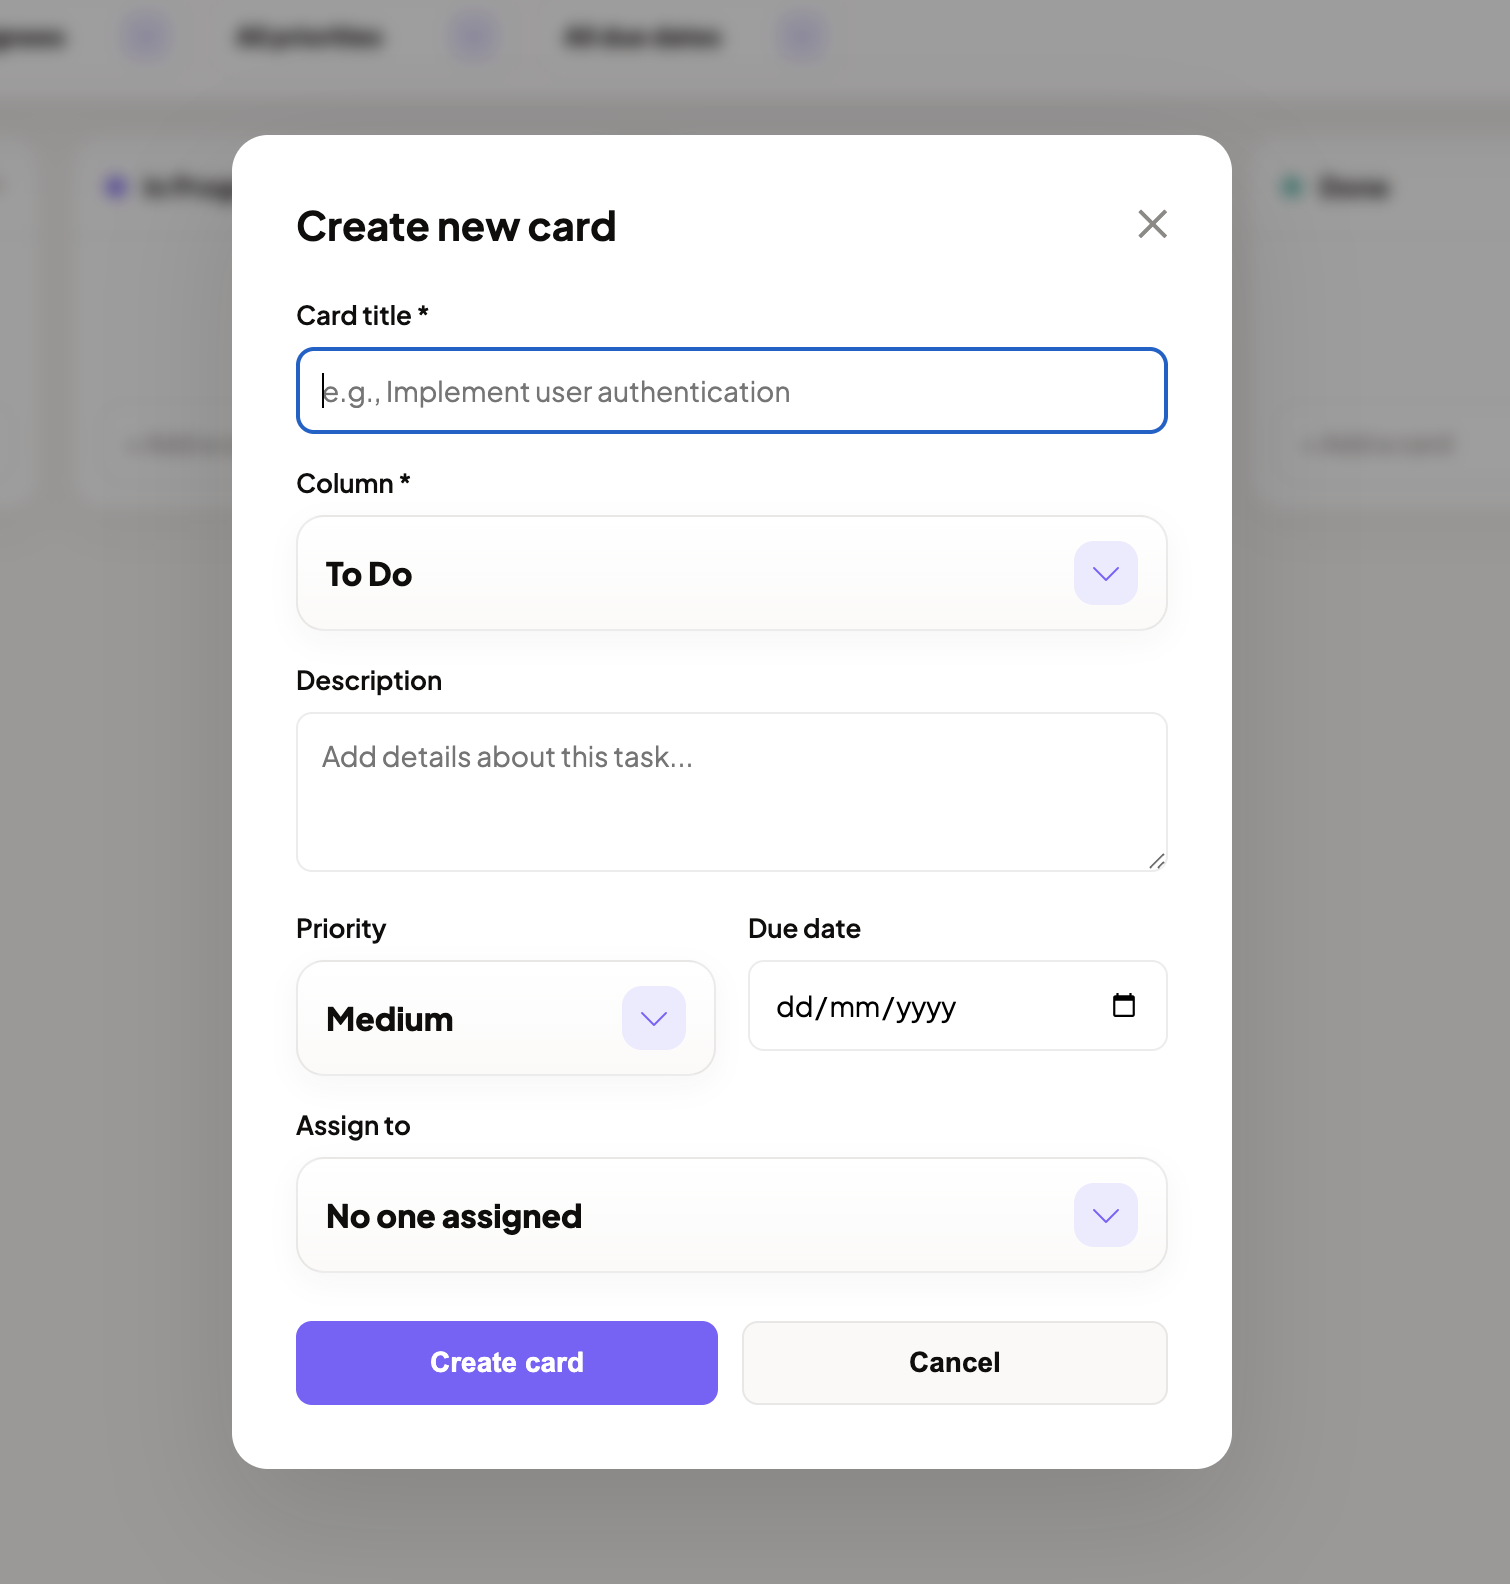
\includegraphics[keepaspectratio,alt={Create-card modal}]{screenshots/report-create-card.png}}
\caption{Create-card modal}
\end{figure}

\subsection{Core Functional Modules}\label{core-functional-modules}

\subsubsection{Workspaces}\label{workspaces}

Users can create workspaces with a name, description, and tech stack.
Each workspace has an owner and an invite code. Workspaces contain
members with roles. Owners/admins can invite users, update roles, and
remove eligible members. The system also supports joining through an
invite code and joining through a secure email invite token.

\subsubsection{Boards and Columns}\label{boards-and-columns}

Each workspace can contain boards, but a newly created workspace starts
empty so the user can decide whether to create a board or join an
existing workspace. Owners and admins can create, update, and delete
boards and columns. When a board is created, the backend adds the
default workflow columns: \texttt{To\ Do}, \texttt{In\ Progress},
\texttt{In\ Review}, and \texttt{Done}.

\subsubsection{Cards}\label{cards}

Cards represent tasks. A card stores:

\begin{itemize}
\tightlist
\item
  title
\item
  description
\item
  priority
\item
  assignee
\item
  due date
\item
  column id
\item
  position
\end{itemize}

Members and above can create, update, delete, and move cards. The
backend validates that a card belongs to the correct board before
allowing updates. When a card is assigned to another user, the system
creates a notification for that user.

\subsubsection{Drag-and-Drop Movement}\label{drag-and-drop-movement}

The frontend uses HTML drag-and-drop events. When a card is dropped into
another column, the frontend calls:

\begin{Shaded}
\begin{Highlighting}[]
\NormalTok{PATCH /api/boards/:boardId/cards/:cardId/move}
\end{Highlighting}
\end{Shaded}

The backend validates access, verifies source and destination columns,
recalculates positions, saves the card, creates an activity entry,
notifies the assignee if required, and emits \texttt{card:moved} to the
board room.

\subsubsection{Comments and Mentions}\label{comments-and-mentions}

TeamOps supports:

\begin{itemize}
\tightlist
\item
  Card comments.
\item
  Board comments.
\item
  Board comment tagged cards.
\item
  Board comment tagged members.
\end{itemize}

Tagged members receive important notifications. The backend normalizes
tagged ids to ensure that only cards from the current board and members
from the current workspace can be referenced.

\subsubsection{Activity and Audit}\label{activity-and-audit}

Every important action can create an activity record. The project
separates normal collaboration activity from governance-sensitive
activity. Governance-related events include workspace, invite, member,
role, permission, login, password, profile, account, security, and
deletion events. Owners and admins can view broader audit logs, while
members/viewers see limited events.

\subsubsection{Notifications}\label{notifications}

Notifications are created for assignments, mentions, moved assigned
cards, and other important events. The inbox supports:

\begin{itemize}
\tightlist
\item
  unread count
\item
  mark one notification as read
\item
  mark all as read
\item
  important flag toggle
\item
  real-time \texttt{notification:new} delivery
\end{itemize}

\subsubsection{Analytics}\label{analytics}

The board analytics endpoint calculates:

\begin{itemize}
\tightlist
\item
  cards per column
\item
  completed cards this week
\item
  cards per assignee
\item
  overdue card count
\end{itemize}

This gives the dashboard measurable project status without requiring a
separate analytics database.

\subsubsection{Dashboard and Saved
Views}\label{dashboard-and-saved-views}

The dashboard has grown into a complete workspace command center. In
addition to the live board, it includes pages for projects, roadmap,
integrations, communication channels, help, saved views, members,
settings, profile, notifications, activity, analytics, and audit logs.
Saved views allow a user to preserve useful board filters locally so
repeated workflows can be reopened quickly.

\subsubsection{Workspace Settings and
Automation}\label{workspace-settings-and-automation}

Owners and admins can adjust workspace automation settings such as
desktop notification preferences, review nudges, escalation days, weekly
digest behavior, after-hours mention filtering, and completed-card
cleanup. The backend normalizes these settings, persists them on the
workspace, runs supported automation actions, and emits
\texttt{workspace:settings} so connected clients can refresh the visible
settings state.

\subsubsection{Profile and My Work}\label{profile-and-my-work}

Users can view and update profile details, upload an avatar, change
password, and see cards assigned to them across accessible boards. This
makes the app useful from both manager and individual contributor
perspectives.

\subsection{Key Algorithms and Logic}\label{key-algorithms-and-logic}

\subsubsection{Cookie-Based JWT
Authentication}\label{cookie-based-jwt-authentication}

The backend signs tokens using:

\begin{Shaded}
\begin{Highlighting}[]
\NormalTok{payload: \{ userId \}}
\NormalTok{expiry: 7 days}
\NormalTok{secret: JWT\_SECRET}
\end{Highlighting}
\end{Shaded}

The JWT is stored in the \texttt{teamops\_session} HTTP-only cookie.
Every protected route requires that cookie. The middleware verifies the
token and sets \texttt{req.userId}. For unsafe methods such as POST,
PATCH, and DELETE, authenticated requests also include the
\texttt{X-CSRF-Token} header matching the readable
\texttt{teamops\_csrf} cookie.

\subsubsection{Role Resolution}\label{role-resolution}

For a request involving a board, column, or card, the backend resolves
the workspace id. Then it checks whether the current user is present in
\texttt{workspace.members} and has the required role.

\subsubsection{Card Positioning}\label{card-positioning}

When a card moves:

\begin{enumerate}
\def\labelenumi{\arabic{enumi}.}
\tightlist
\item
  Load the card.
\item
  Load source column and target column.
\item
  Verify both columns belong to the current board.
\item
  Remove the moved card from the destination list if it is already
  there.
\item
  Insert the card at the target index.
\item
  Save the destination cards with updated positions.
\item
  Recalculate source column positions if the card changed columns.
\item
  Emit a real-time event and return success.
\end{enumerate}

\subsubsection{Due Date Rule}\label{due-date-rule}

The backend prevents active cards from being assigned a due date in the
past. A past due date is allowed if the card is already in a
\texttt{Done} column, or when preserving an existing historical date.
This avoids accidental invalid scheduling while still allowing completed
historical work.

\subsubsection{Activity Visibility}\label{activity-visibility}

Activity filtering uses a governance pattern. Owners/admins can see
governance events. Members/viewers only see governance events they
personally caused, while normal board collaboration remains visible.

\subsection{Security Considerations}\label{security-considerations}

{\def\LTcaptype{} % do not increment counter
\begin{longtable}[]{@{}
  >{\raggedright\arraybackslash}p{(\linewidth - 2\tabcolsep) * \real{0.5000}}
  >{\raggedright\arraybackslash}p{(\linewidth - 2\tabcolsep) * \real{0.5000}}@{}}
\toprule\noalign{}
\begin{minipage}[b]{\linewidth}\raggedright
Area
\end{minipage} & \begin{minipage}[b]{\linewidth}\raggedright
Current Implementation
\end{minipage} \\
\midrule\noalign{}
\endhead
\bottomrule\noalign{}
\endlastfoot
Password storage & bcrypt hashing, no plain password storage \\
Session auth & JWT stored in HTTP-only cookie with server-side
verification \\
CSRF protection & Double-submit CSRF cookie/header for unsafe
authenticated requests \\
Email verification & OTP stored with expiry \\
Password reset & OTP reset code with expiry \\
Google login & Google ID token verification \\
Authorization & Workspace role checks in middleware and controllers \\
Input validation & Required fields, trimmed values, role validation,
date validation \\
CORS & Configurable origin allowlist with local dev support \\
Data scoping & Board/column/card operations verify workspace
membership \\
Realtime privacy & Socket.io reads the session cookie and user
notifications emit to \texttt{user:\textless{}userId\textgreater{}}
room \\
\end{longtable}
}

Potential improvements:

\begin{itemize}
\tightlist
\item
  Enforce a stronger \texttt{JWT\_SECRET} in all environments.
\item
  Add rate limiting for login, verification, and reset endpoints.
\item
  Hash OTP/reset tokens before storing them.
\item
  Add server-side file storage instead of base64 avatars.
\item
  Add account lockout controls for repeated failed auth attempts.
\item
  Add schema-level indexes for common analytics and activity queries.
\item
  Add automated tests for auth, RBAC, board movement, and invite flows.
\item
  Use Redis adapter if Socket.io needs multiple backend instances.
\end{itemize}

\subsection{Testing and Verification}\label{testing-and-verification}

The repository does not include a formal automated test suite, but it
includes useful verification commands:

Backend:

\begin{Shaded}
\begin{Highlighting}[]
\BuiltInTok{cd}\NormalTok{ teamops{-}backend}
\ExtensionTok{npm}\NormalTok{ test}
\end{Highlighting}
\end{Shaded}

The backend \texttt{test} script currently runs
\texttt{node\ -\/-check\ server.js}, which verifies JavaScript syntax
for the entry file.

Frontend:

\begin{Shaded}
\begin{Highlighting}[]
\BuiltInTok{cd}\NormalTok{ teamops{-}frontend}
\ExtensionTok{npm}\NormalTok{ run lint}
\ExtensionTok{npm}\NormalTok{ run build}
\end{Highlighting}
\end{Shaded}

The frontend \texttt{test} script runs lint and build. Because the
active app is standalone HTML/JS, manual testing is still important.

\subsection{Future Enhancements}\label{future-enhancements}

\begin{enumerate}
\def\labelenumi{\arabic{enumi}.}
\tightlist
\item
  Add automated backend tests with Jest or Node's built-in test runner.
\item
  Add Playwright end-to-end tests for authentication, board CRUD,
  movement, and invites.
\item
  Add file attachments to cards using cloud storage.
\item
  Add recurring tasks and task templates.
\item
  Add Redis adapter for multi-instance Socket.io scaling.
\item
  Add rate limiting and audit hardening for auth routes.
\item
  Add advanced reports such as burndown charts and cycle time.
\item
  Add email notification preferences connected to backend settings.
\item
  Add mobile-friendly refinements and PWA support.
\item
  Split frontend logic into smaller modules while keeping the no-React
  architecture if required.
\end{enumerate}

\subsection{Conclusion}\label{conclusion}

TeamOps successfully demonstrates a full-stack real-time collaboration
platform. It combines authentication, authorization, database design,
REST APIs, WebSocket events, frontend state rendering, Kanban workflows,
notifications, activity logging, and analytics in one coherent project.
The most important technical achievement is that the app is not just a
static dashboard: actions on boards are persisted in MongoDB, scoped by
workspace permissions, logged as activities, and broadcast to connected
users through Socket.io.

The project is suitable for a project submission because it covers core
software engineering topics: requirements analysis, system architecture,
schema design, API design, security, real-time communication, UI
implementation, testing strategy, and future work.

\subsection{Appendix A: Important API
Endpoints}\label{appendix-a-important-api-endpoints}

{\def\LTcaptype{} % do not increment counter
\begin{longtable}[]{@{}
  >{\raggedright\arraybackslash}p{(\linewidth - 4\tabcolsep) * \real{0.3333}}
  >{\raggedright\arraybackslash}p{(\linewidth - 4\tabcolsep) * \real{0.3333}}
  >{\raggedright\arraybackslash}p{(\linewidth - 4\tabcolsep) * \real{0.3333}}@{}}
\toprule\noalign{}
\begin{minipage}[b]{\linewidth}\raggedright
Method
\end{minipage} & \begin{minipage}[b]{\linewidth}\raggedright
Endpoint
\end{minipage} & \begin{minipage}[b]{\linewidth}\raggedright
Purpose
\end{minipage} \\
\midrule\noalign{}
\endhead
\bottomrule\noalign{}
\endlastfoot
POST & \texttt{/api/auth/register} & Register new user \\
POST & \texttt{/api/auth/verify} & Verify email OTP \\
POST & \texttt{/api/auth/login} & Login with email/password \\
POST & \texttt{/api/auth/google} & Login using Google credential \\
POST & \texttt{/api/auth/forgot-password} & Start reset flow \\
POST & \texttt{/api/auth/reset-password} & Reset password using OTP \\
POST & \texttt{/api/auth/logout} & Clear session and CSRF cookies \\
GET & \texttt{/api/workspaces} & List user's workspaces \\
POST & \texttt{/api/workspaces} & Create workspace \\
POST & \texttt{/api/workspaces/join} & Join workspace using invite
code \\
GET & \texttt{/api/workspaces/join/invite} & Accept secure email invite
token \\
GET & \texttt{/api/workspaces/:workspaceId/boards} & List boards in
workspace \\
POST & \texttt{/api/workspaces/:workspaceId/boards} & Create board \\
POST & \texttt{/api/workspaces/:workspaceId/invite-email} & Send
workspace email invite \\
GET & \texttt{/api/workspaces/:workspaceId/automation-settings} & Load
workspace automation settings \\
PATCH & \texttt{/api/workspaces/:workspaceId/automation-settings} &
Update workspace automation settings \\
GET & \texttt{/api/boards/:boardId} & Get board with columns/cards \\
GET & \texttt{/api/boards/:boardId/analytics} & Get board analytics \\
POST & \texttt{/api/boards/:boardId/cards} & Create card \\
PATCH & \texttt{/api/boards/:boardId/cards/:cardId} & Update card \\
PATCH & \texttt{/api/boards/:boardId/cards/:cardId/move} & Move card \\
DELETE & \texttt{/api/boards/:boardId/cards/:cardId} & Delete card \\
GET & \texttt{/api/activities/workspace/:workspaceId/audit} & Get admin
audit log \\
GET & \texttt{/api/notifications} & Notification inbox \\
GET & \texttt{/api/user/profile} & User profile \\
PATCH & \texttt{/api/user/profile} & Update profile \\
\end{longtable}
}

\end{document}
